\chapter{The universal symmetry: the circle}
\label{cha:circle}

An effective principle in mathematics is that when you want to study a certain
phenomenon you should search for a single type that captures this phenomenon.
Here are two examples:\footnote{%
  Notice that these have arrows pointing in different directions:
  In~\cref{it:one-out} we're mapping \emph{out} of $\bn{1}$,
  while in~\cref{it:prop-in} we're mapping \emph{in} to $\Prop$.}
\begin{enumerate}
\item\label{it:one-out}
  The contractible type $\bn 1$ has the property that given
any type $A$ a function $\bn 1\to A$ provides exactly the
same information as picking an element in $A$.
For, an equivalence from $A$ to $\bn 1\to A$ is provided by
the function $a \mapsto (x \mapsto a)$, see \cref{xca:Xequiv1toX}.
\item\label{it:prop-in}
  The type $\Prop$ of propositions has the property that
given any type $A$ a function $A\to\Prop$ provides exactly
the same information as picking a subtype of $A$,
see \cref{lem:Prop-Set-pointed-families}(\ref{lem:Prop-families}).
\end{enumerate}
We are interested in symmetries, and so we should search for a type $X$
which is so that given \emph{any} type $A$ the type of functions
$X\to A$ (or $A\to X$, but that's not what we're going to do)
picks out exactly the symmetries in $A$.
We will soon see that there is such a type:
the circle\footnote{%
  We call this type the ``circle''
  because it has many properties which are analogues, in our context, of properties of
  the topological circle $\setof{(x,y)\in\RR^2}{x^2+y^2=1}$.
  See~\cref{sec:topology} for a discussion of the relationship
  between topological spaces and types.
  In the later chapters on geometry we'll return
  to ``real'' geometrical circles.}
which is built \emph{exactly} so that this
``universality with respect to symmetries'' holds.
It may be surprising to see how little it takes to define it;
especially in hindsight when we eventually discover some of the many uses of the circle.

A symmetry in $A$ is an identification $p:a\eqto a$ for some $a:A$.%
\index{symmetry!in a type}
Now, we can take any iteration of $p$ (composing $p$ with itself a number of times),
and we can consider the inverse $p^{-1}$ and \emph{its} iterations.
So, by giving one symmetry we give at the same time a lot of symmetries.
For a particular $p: a\eqto a$ it may be that some of the iterations
can be identified (in their type $a\eqto a$). For instance, it may be
that there is an identification of type $p^2 \eqto p^0$ (as in \cref{xca:C2}).
Even more dramatically: if there is an identification of type
$p\eqto\refl a$, then \emph{all} the
iterations of $p$ can be identified with each other.\marginnote{%
  \begin{tikzpicture}
    \node (A) at (0,-1.5) {$A$};
    \begin{scope}[thick]
      \draw (0,-1)
      .. controls ++(200:-1) and ++(180:1) .. (2,-2)
      .. controls ++(180:-1) and ++(270:1) .. (4,0)
      .. controls ++(270:-1) and ++(10:1)   .. (2,2.25)
      .. controls ++(10:-1)   and ++(90:1)  .. (-.5,1)
      .. controls ++(90:-1)  and ++(200:1) .. (0,-1);
      \pgfmathsetmacro\gsize{3}%
      \pgfmathsetmacro\gscale{min(1,\gsize/4)}%
      \pgfmathsetmacro\gyscale{0.25*\gscale*.707}%
      \pgfmathsetmacro\gxscale{0.5*\gscale}%
      \pgfmathsetmacro\gsep{((\gsize - 2*\gscale)/2*0.5)}%
      \pgfmathsetmacro\omrstwo{1 - 1/sqrt(2)}%
      \pgfmathsetmacro\sqrtwo{sqrt(2)}%
      \draw (1 + \gsep +  \gxscale + \gxscale -\omrstwo*\gxscale,0)
      .. controls +(-\gxscale*\sqrtwo/3,4/3*\gyscale)
      and +(\gxscale*\sqrtwo/3,4/3*\gyscale)
      .. ++(-\sqrtwo*\gxscale,0);
      \draw (1 + \gsep +  \gxscale - \gxscale,0 + \gyscale)%
      .. controls +(\gxscale*2/3,-8/3*\gyscale)
      and +(-\gxscale*2/3,-8/3*\gyscale)
      .. ++(2*\gxscale,0);
    \end{scope}
    \begin{scope}[shift={(-1.25,-7.25)}]
      \node[dot,label=right:$a$] (a) at (1.99,7.58) {};
      \draw[->]
      (4.02,7.58) .. controls (3.97,8.13) and (3.93,8.66) .. node[auto,swap] {$p$}
      (3.07,8.60) .. controls (2.20,8.54) and (1.99,8.00) ..
      (1.99,7.58) .. controls (1.98,7.15) and (2.25,6.67) ..
      (2.97,6.56) .. controls (3.70,6.44) and (4.06,7.03) ..
      (4.02,7.58);
      \draw[casblue,->]
      (3.25,6.44) .. controls (4.01,6.46) and (4.59,7.71) ..
      (3.77,8.45) .. controls (2.95,9.20) and (1.83,8.42) ..
      (1.81,7.60) .. controls (1.79,6.78) and (3.00,5.63) ..
      (3.94,6.67) .. controls (4.88,7.71) and (4.02,8.50) ..
      (3.54,8.78) .. controls (3.05,9.05) and (1.99,8.45) .. node[auto,swap] {$p^2$}
      (1.99,7.58) .. controls (1.99,6.70) and (2.49,6.42) ..
      (3.25,6.44);
      \draw[casred,->]
      (3.12,8.52) .. controls (3.69,8.49) and (3.81,8.27) ..
      (3.87,7.75) .. controls (3.93,7.23) and (3.67,6.58) ..
      (2.95,6.65) .. controls (2.23,6.71) and (1.98,7.01) ..
      (1.99,7.58) .. controls (2.00,8.14) and (2.55,8.55) ..
      node[auto,swap] {$p^{-1}$}
      (3.12,8.52);
    \end{scope}
  \end{tikzpicture}}
However, in general we must be prepared that all the iterations $p_n$
of $p$ (for $n$ positive, $0$ and negative) are distinct.
Hence, the circle must have a distinct symmetry for every integer.
We would have enjoyed defining the integers this way,
but being that ideological would be somewhat inefficient.
Hence we give a more hands-on approach and define the circle
and the integers separately. Thereafter we prove that the type of
symmetries in the circle is equivalent to the set of integers.

\section{The circle and its universal property}
\label{sec:S1}

Propositional truncation from \cref{sec:prop-trunc} was
the first \emph{higher inductive type}, that is, an inductive type
with constructors both for elements and for identifications,
we introduced.
The circle is another example of a higher inductive type,
see Chapter~6 of the HoTT book\footcite{hottbook} for more information.

\begin{definition}
  \label{def:circle}
The circle is a type $\Sc:\UU$ with an element (constructor) $\base : \Sc$ and
an identification (constructor) ${\Sloop}: \base\eqto\base$. For convenience and
clarity the (higher) induction principle for $\Sc$ is explained
by first stating a recursion principle for $\Sc$.

Let $A$ be a type. In order to define a function $f:\Sc\to A$,
it suffices to give an element $a$ of $A$ together with an
identification $l$ of type $a \eqto a$. The function $f$ defined
by this data satisfies $f(\base)\jdeq a$ and
the recursion principle provides an identification of type
$\ap{f}(\Sloop)=l$.

\begin{marginfigure}
  \noindent\begin{tikzpicture}
    \node (A) at (2,3) {$\sum_{x:\Sc}A(x)$};
    \node (Sc) at (2,0) {$\Sc$};
    \node (Sloop) at (.9,-.5) {$\Sloop$};
    \draw[->] (A) -- node[auto] {$\fst$} (Sc);
    \draw[->] (-90:1 and .3) arc (-90:270:1 and .3);
    \node[basedot] at (-1,0) {};
    % then: A top and bottom
    \coordinate[label=above left:$A(\base)$] (A-top-left) at (-1,2.7);
    \coordinate (A-bot-left) at (-1,0.9);
    \coordinate (A-top-front) at (0,2.4);
    \coordinate (A-bot-front) at (0,0.7);
    \coordinate (A-top-back) at (0,2.8);
    \coordinate (A-bot-back) at (0,1.3);
    \coordinate (A-top-right) at (1,2.6);
    \coordinate (A-bot-right) at (1,0.8);
    \draw (A-top-left) -- (A-bot-left)
    .. controls +(-90:.3) and +(-10:-.5) .. (A-bot-front)
    .. controls +(-10:.5) and +(90:-.3) .. (A-bot-right)
    -- (A-top-right)
    .. controls +(-90:.2) and +(170:-.5) .. (A-top-front)
    .. controls +(170:.5) and +(90:-.2) .. (A-top-left);
    \draw[dashed] (A-bot-left)
    .. controls +(90:.3) and +(5:-.4) .. (A-bot-back)
    .. controls +(5:.4) and +(-90:-.3) .. (A-bot-right);
    \draw (A-top-left)
    .. controls +(90:.3) and +(-10:-.3) .. (A-top-back)
    .. controls +(-10:.3) and +(-90:-.3) .. (A-top-right);
    \node[dot,label=left:$a$] (a-left) at (-1,2) {};
    \coordinate (a-front) at (0,1.6);
    \coordinate (a-right) at (1,1.8);
    \coordinate (a-back) at (0,2.2);
    \draw[->] (a-left)
    .. controls +(-90:.3) and +(-15:-.4) .. (a-front);
    \draw (a-front)
    .. controls +(-15:.4) and +(90:-.3) .. node[auto] {$l$} (a-right);
    \draw[dashed] (a-left)
    .. controls +(90:.3) and +(-5:-.4) .. (a-back)
    .. controls +(-5:.4) and +(-90:-.3) .. (a-right);
  \end{tikzpicture}
  \caption{The induction principle of $\Sc$.}
  \label{fig:circle-induction}
\end{marginfigure}

Let $A(x)$ be a family of types parametrized by the variable $x:\Sc$.
The induction principle of $\Sc$ states that, in order to define a family
of elements of $A(x)$ parametrized by the variable $x:\Sc$,
it suffices to give an element $a$ of $A(\base)$ together with an
identification $l$ of type $\pathover{a}{A}{\Sloop}{a}$,
see \cref{fig:circle-induction}.
The function $f : \prod_{x:\Sc}A(x)$ defined by this
data satisfies $f(\base)\jdeq a$ and the induction principle
provides an identification of type $\apd{f}(\Sloop) \eqto l$.
\end{definition}

Giving $a$ as above is referred to as `the base case', and
giving $l$ as `the loop case'. Given this input data to define
a function $f$ will often be abbreviated by writing
$f(\base)\defeq a$ and $f(\Sloop)\defis l$.  Notice the use of $\defis$\glossary(2:=){$\defis$}{identification in a definition} in the
second definition, instead of $\defeq$.  That signifies that $f(\Sloop)$ and
$l$ are not equal by definition, but rather, that an identification is given between
them, i.e., an element of type $f(\Sloop) \eqto l$ is given, or an element of
$\apd{f}(\Sloop) \eqto l$ is given, in the dependent case.

The following result states that any function from the circle exactly
picks out an element and a symmetry of that element.
This is a ``universal property'' of the circle.

\begin{theorem}\label{lem:freeloopspace}
For all types $A$, the evaluation function
\[
\ev_A : (\Sc\to A)\to \sum_{a:A}(a\eqto a)\text{~defined by~}
\ev_A(g)\defeq (g(\base),g(\Sloop))
\]
is an equivalence, with inverse $\ve_A$ defined by the recursion principle
of the circle.
\end{theorem}
\begin{proof}
Fix $A:\UU$. We apply \cref{lem:weq-iso}.
For all $a:A$ and $l:a\eqto a$ we may construct an identification of type $\ev(\ve(a,l))\eqto(a,l)$
by the recursion principle. It remains to construct identifications
of type $\ve(\ev(f))\eqto f$ for all $f:\Sc\to A$.  Such constructions are provided by
the following more general result.
Given $f,g:\Sc\to A$,
$p: f(\base)\eqto g(\base)$, and $q: f(\Sloop) \eqto p^{-1}\cdot g(\Sloop)\cdot p$,
we construct an identification of type $f\eqto g$, as follows.
It suffices, by function extensionality, to construct an element of
type $P(x)\defeq(f(x)\eqto g(x))$ for a variable $x:\Sc$.
This we do by circle induction.
For the base case we take $p$.
The loop case reduces to constructing an identification of type $\trp[P]{\Sloop}(p)\eqto p$, by \cref{def:pathover-trp}.
By \cref{lem:trp-in-fx=Ygx} we have an identification of type
$\trp[P]{\Sloop}(p)\eqto g(\Sloop)\cdot p \cdot f(\Sloop)^{-1}$.
Using $q$ we construct an identification of type $g(\Sloop) \eqto p\cdot f(\Sloop) \cdot p^{-1}$.
Hence we may construct an identification of type $\trp[P]{\Sloop}(p)\eqto p$, by an easy calculation.
Now apply \cref{lem:isEq-pair=}, and we have
constructed a function of type $(\ev(f)\eqto \ev(g)) \to (f\eqto g)$.

Now we get an identification of type $\ve(\ev(f))\eqto f$, for we have an identification of type
$\ev(\ve(\ev(f)))\eqto (f(\base),f(\Sloop))$, and $(f(\base),f(\Sloop))\jdeq\ev(f)$,
with $p\defeq\refl{f(\base)}$ and $q$ coming from the induction principle.
\end{proof}
\begin{corollary}\label{cor:circle-loopspace}
  For any $a:A$, the function
  \[\ev_A^a:((\Sc,\base)\to_* (A,a))\to (a\eqto a)\]
  sending $(g,p)$ to $p^{-1}\cdot g(\Sloop)\cdot p$ is an equivalence.
\end{corollary}
\begin{proof}\hskip-5pt\footnote{%
    This can also be done directly:
    The inverse to $\ev_A^a$ sends $l : a\eqto a$
    to $(\ve_A(a,l), \refl{a})$.
    Try to verify this!}
Consider the following diagram (see \cref{rem:diagram}):
\[
  \begin{tikzcd}
    (\Sc \to A) \ar[rr,"{g\mapsto(g(\base),g,\refl{g(\base)})}"]
    \ar[dr,"\ev_A"'] & &
    \sum_{a:A}\bigl((\Sc,\base) \ptdto (A,a)\bigr)
    \ar[dl,"\tot(\ev_A^-)"] \\
    &  \,\sum_{a:A}(a\eqto a),
  \end{tikzcd}
\]
where the top map is an equivalence by \cref{cor:contract-away},
and the left map is an equivalence by \cref{lem:freeloopspace}.
This diagram represents the identity type $\ev_A \eqto
(g\mapsto (g(\base),\inv{\refl{g(\base)}}\cdot g(\Sloop)\cdot\refl{g(\base)}))$.
An identification of this type is provided by function
extensionality and \cref{xca:path-groupoid-laws}.
The result now follows from \cref{lem:fiberwise-equiv-from-tot}.
\end{proof}

\begin{remark}\label{rem:dep-univ-prop-circle}
By almost the same argument as for \cref{lem:freeloopspace}
one can obtain the dependent universal property of the circle.
Given a type family $A:\Sc\to\UU$, the dependent evaluation function,
which also maps $g$ to $(g(\base),g(\Sloop))$ but has type
$(\prod_{x:\Sc} A(x))\to \sum_{a:A(\base)}(\pathover a A {\Sloop} a)$,
is an equivalence. (Compare the latter type to the type of $\ev_A$
in \cref{lem:freeloopspace} and see \cref{fig:circle-induction}.)
\end{remark}

\begin{marginfigure}
  \begin{tikzpicture}
    %% draw S1
    \node[dot,label=below:$\Sc$] (base) at (0,0) {};%
    \draw[->] (base) .. controls ++(45:1) and ++(135:1) .. node (loop)
    {} (base);
    %% type A
    \begin{scope}[xshift=5em]
      \draw plot [smooth cycle] coordinates {(0,0) (1.5,0) (1.3,1)
        (0,1.5)};%
      \node[dot,label=below:$a$] (a) at (.5,.5) {};%
      \node (A1) at (1.5,1.5) {$A$}; \draw[->] (a) .. controls
      ++(-20:1) and ++(-30:.5) .. ++(45:.5) .. controls ++(150:1) and
      ++(210:1) .. node[very near start] (middle) {} (a);
    \end{scope}
    %% draw map f
    \draw[dashed, ->, shorten <= 3pt, shorten >= 3pt] (loop) to[bend
    left] node[above]{$f$} (middle);
  \end{tikzpicture}
\end{marginfigure}
\begin{remark}
  A function $f:\Sc\to A$ is often called a \emph{loop} in $A$, the
  picture being that $f$ throws $\Sloop:\base\eqto\base$ as a lasso in the
  type $A$.

  Using the equivalence in \cref{cor:circle-loopspace} and univalence,
  $a\eqto a$ is identified with the pointed
  functions from the circle, which allows for a very graphic
  interpretation of the symmetries of $a$ in $A$: they are traced out
  by a function $f$ from the circle and can be seen as loops in the type
  $A$ starting and ending at $a$!\footnote{%
    This is of course how we have been
    picturing loops the whole time.}
\end{remark}

\begin{lemma}\label{lem:circleisconnected}
  The circle is connected.
\end{lemma}
\begin{proof}
We show $\Trunc{\base\eqto z}$ for all $z:\Sc$ by circle induction
as in \cref{def:circle}.
For the base case we take $\trunc{\refl{\base}}:\Trunc{\base\eqto \base}$.
The loop case is immediate as $\Trunc{\base\eqto \base}$ is a proposition.
\end{proof}

In the proof above, the propositional truncation coming
from the definition of connectedness is essential.
If this truncation were removed we wouldn't know what to do in
the induction step (actually, having an element of type
$\prod_{z:\Sc}(\base\eqto z)$ contradicts the univalence axiom).
This said, the family $R:\Sc\to\UU$ with $R(z)\defequi (\base\eqto z)$
is extremely important for other purposes. In \cref{def:universalcover},
we will call $R$ the ``universal \covering'' of the circle,
and it is the key tool in proving that the type of symmetries in
the circle is a set that can be identified with the set of integers.
Recall that we
use the phrase ``symmetries \emph{in} the circle'' to refer to the
elements of $\base\eqto\base$,\footnote{%
  Here we are using ``the circle'' to mean the
  \emph{pointed} type $(\Sc,\base)$.
  But it also turns out that the type $\base\eqto\base$ is
  equivalent to the type $x\eqto x$, for any $x:\Sc$.}
whereas we use the phrase ``symmetries \emph{of} the circle'' to
refer to the elements of $\Sc\eqto_\UU\Sc$.
The latter type is equivalent to $\Sc\amalg\Sc$,
as follows from \cref{xca:S1=S1-components} and \cref{{xca:(S1->S1)_(f)-eqv-S1}}.

In order to proceed, we should properly define the set of integers
and explore the concept of \coverings.

\section{The integers}
\label{sec:integers}

We define the type of integers in one of the many possible ways.\footnote{%
  \label{ft:many-integers}Here are some of these alternatives:
  \begin{itemize}
  \item As the copy of $\NN$ where $2n$ means $n$ and $2n+1$ means $-n-1$, for $n:\NN$.
  \item As the sum $\NN\coprod\NN$, where $\inl{n}$ means $-n-1$ and $\inr{n}$ means $n$.
  \item As the sum $\NN\coprod\bn1\coprod\NN$, where from the left copy of $\NN$ we get $-n-1$, from the center $0:\bn1$ we get $0$, and from the right copy of $\NN$ we get $n+1$, for $n:\NN$.
  \item As the quotient of $\NN\times\NN$ under the equivalence relation
    $(n,m) \sim (n',m')$ defined by $n+m' = n'+m$,
    where $(n,m)$ represents $n-m$.
  \item As the subset of $\NN\times\NN$ consisting of those $(n,m)$ with $n=0\lor m=0$ (picking canonical representatives for the above equivalence relation).
  \item As the loops $\base\eqto\base$ in the circle. %$\ddot\smile$
  \end{itemize}}

\begin{definition}\label{def:zet}
  Let $\zet$ be the higher inductive type with the following three
  constructors:\glossary(Z){$\protect\zet$}{the set of integers,
  \cref{def:zet}}
\begin{enumerate}
\item $\iota_+: \NN \to \zet$ for the nonnegative numbers,
  $0,1,\ldots$\glossary(909iota+){$\iota_+$}{embedding of $\NN$ into $\zet$}
\item $\iota_-: \NNN \to \zet$ for the nonpositive numbers,
  $-0,-1,\ldots$\glossary(909iota-){$\iota_-$}{embedding of $\NNN$ into $\zet$}
\item $\zeq : \iota_-(-0) = \iota_+(0)$.
\end{enumerate}
Because we used the copy $\NNN$ for the nonpositive numbers from \cref{exa:nnn},
we can leave out the constructor symbols $\iota_\pm$
when the type is clear from context.
Thus we have $\ldots,-2,-1,-0,0,1,2,\ldots:\zet$ and $\zeq:-0\eqto_\zet0$.

The type $\zet$ comes with an induction principle:
Let $T(z)$ be a family of types parametrized by $z:\zet$.
In order to construct an element $f(z)$ of $T(z)$ for all $z:\zet$,
it suffices to give functions $g$ and $h$ such
that $g(n): T(\iota_+(n))$ and $h(n): T(\iota_-(m))$ for all $n:\NN,m:\NNN$,
together with $q : \pathover {h(-0)} T \zeq {g(0)}$.
Here $g$ and $h$ can be defined by induction on $n:\NN,m:\NNN$.\footnote{%
  Of course, giving $h$ is the same as giving $h':\prod_{n:\NN}T(-n)$.}

The resulting function $f:\prod_{z:\zet}T(z)$ satisfies
$f(n)\jdeq g(n)$ and $f(-n)\jdeq h(-n)$ for $n:\NN$,
and there is an (unnamed) element of $\apd{f}(\zeq) = q$.
\end{definition}

Like the type $\NN$, the type $\zet$ is a set with decidable equality
and ordering relations.

One well-known self-equivalence is \emph{negation}, ${-}:\zet\to\zet$,
\index{negation!of integer}\glossary(1negation){$-z$}{negation of an integer $z$}
inductively defined by setting
$-\iota_+(n)\defeq \iota_-(-n)$,
$-\iota_-(m)\defeq \iota_+(-m)$,
$\constant{ap}_-(\zeq) \defis \inv{\zeq}$.\footnote{%
  Here we included the constructor symbols for clarity,
  but the definition allows us to use the negation symbol
  unadorned, because the following diagram
  is commutative by definition:
  \[
    \begin{tikzcd}[column sep=large,row sep=large,ampersand replacement=\&]
      \NN \ar[r,shift left=1mm,"-"]\ar[d,"\iota_+"']
      \& \NNN \ar[l,shift left=1mm,"-"]\ar[d,"\iota_-"] \\
      \zet \ar[r,shift left=1mm,"-"]
      \& \zet \ar[l,shift left=1mm,"-"]
    \end{tikzcd}
  \]}
Negation is its own inverse.

The \emph{successor} function $\zs:\zet\to\zet$%
\glossary(s){$\protect\zs$}{successor function on $\zet$} is
likewise defined inductively, setting
$\zs(n) \defeq \Succ(n)$,
$\zs(-0) \defeq 1$,
$\zs(-\Succ(n)) \defeq -n$,
and $\ap{\zs}(\zeq) \defis \refl{1}$.

The successor function $\zs$ is an equivalence.
It is instructive to depict iterating $\zs$ in both directions as
a doubly infinite sequence containing all integers:
\[
  \begin{tikzcd}[arrows=mapsto,row sep=tiny]
    & & & -0 \ar[dd,eqr]\ar[dr] & & & \\
    \cdots\ar[r] & -2\ar[r] & -1\ar[ur] & & 1\ar[r] & 2\ar[r] & \cdots \\
    & & & 0 \ar[ur] & & &
  \end{tikzcd}
\]

The inverse $\inv\zs$ of $\zs$ is called the \emph{predecessor} function.
We recall the $n$-fold iteration $\zs^n$ defined earlier;
the $n$-fold iteration of $\zs^{-1}$ will be denoted by $\zs^{-n}$.
Since $\zs^0 \jdeq \id \jdeq \zs^{-0}$,
this defines the iteration $\zs^z$ for all $z:\zet$.\footnote{%
  In the same way, we can define the iteration
$f^z : X \to X$ for any \emph{equivalence} $f : X \to X$.}\index{iteration}

\emph{Addition} of integers is now defined by iteration:
$z + y \defeq \zs^{y}(z)$.  This extends $+$ on the $\iota_+$-image of
$\NN$, see \cref{xca:addition-on-Z-and-N}.  From addition and
${-}: \zet\to\zet$ one can define a \emph{subtraction} function
setting $z-y \defeq z+(-y)$.
\glossary(2subtraction){${-}$}{subtraction of integers} Since addition
and subtraction are mutually inverse, the function $w\mapsto z+w$ is
an equivalence, and we may iterate it to define \emph{multiplication}:
$zy \defeq (w \mapsto z+w)^y(0)$.

\begin{xca}\label{xca:addition-on-Z-and-N}
  Show that $\iota_+(n+m)=\iota_+(n)+\iota_+(m)$
  and $\iota_+(nm) =\iota_+(n)\iota_+(m)$ for all $n,m:\NN$.
\end{xca}

The ordering relations $<$ and $\leq$ on $\zet$ are easily defined
and shown to extend those on $\NN$.

Recall the induction principle for $\zet$ in \cref{def:zet} above.
Instead of defining $g$ and $h$ explicitly, we will often
give $f(0)$ directly, and
define $g'$ and $h'$ such that $g'(z): T(z)\to T(z+1)$
for all $z:\zet$ with $z\geq 0$, and $h'(z): T(z)\to T(z-1)$
for all $z:\zet$ with $z\leq 0$. The function $f$ thus defined
satisfies $f(-0) \jdeq f(0)$,
$f(z+1)\jdeq g'(z,f(z))$ for all $z\geq 0$,
and $f(z-1)\jdeq h'(z,f(z))$ for all $z\leq 0$.

\begin{xca}\label{xca:commutative-add-Z}
  Show that $x+y = y+x$ and $xy=yx$ for all $x,y:\zet$.
\end{xca}

\section{\Coverings}
\label{sec:covering}

As mentioned earlier, it is possible to define the integers as the
type $\base\eqto\base$ of symmetries in the circle.
Our investigation of $\base\eqto\base$ will use the concept of \coverings.
Since we are going to return to this concept several times,
we take the time for a fuller treatment before we continue with
proving the equivalence of $\base\eqto\base$ and $\zet$.

\begin{definition}\label{def:covering}
A \emph{\covering} over a type $B$
is a map $f:A\to B$ such that for each $b:B$ the preimage 
(fiber) $f^{-1}(b)$ is a set.
We say that a \covering $f:A\to B$ over $B$ is
\begin{itemize}
\item \emph{connected}\index{connected \covering} if $A$ is connected,
%\item \emph{universal}\index{universal \covering} if $A$ and all
%the identity types $a\eqto a$ (for $a:A$) are connected,
\item \emph{finite}\index{finite \covering} if all preimages are finite sets,
\item \emph{decidable}\index{decidable \covering} if all preimages are decidable sets.
\end{itemize}

If $A$ and $B$ are pointed types, a \emph{pointed} \covering is a pointed map
$f:A\to_*B$ such that, when forgetting the points, $f_\div:A_\div\to B_\div$
is a \covering. Here it suffices that $A$ is a pointed type.\footnote{%
  Given a pointed type $(A,a)$, a type $B$ and a map $f : A \to B$,
  $(f,\refl{f(a)}) : (A,a) \ptdto (B,f(a))$ is a pointed map.
  Indeed, the forgetful map $\bigl(\sum_{b:B}((A,a)\ptdto(B,b))\bigr)
  \to (A \to B)$ is an equivalence by \cref{cor:contract-away}.}

We do not require the preimages of $f_\div$ to be pointed types.
\end{definition}
With a formula, given a type $B$, the type of \coverings over $B$ is
\[
\SetBundle(B) \defeq \sum_{A:\UU}\sum_{f:A\to B}\prod_{b:B}\isset(f^{-1}(b)),
\]
with variations according to the flavor.

Recall the equivalence in \cref{lem:Prop-Set-pointed-families}\ref{lem:Set-families}
between the type $B\to\Set$ of families of sets parametrized by elements of $B$, and the type
of \coverings over $B$ given above.
We shall frequently use this equivalence, even without explicit mention.

\begin{lemma}\label{lem:setbundle-is-groupoid}
For any type $B$, $\SetBundle(B)$ is a groupoid.
\end{lemma}
\begin{proof}
By \cref{lem:Set-is-groupoid} we have that $\Set$ is a groupoid,
and hence $B\to\Set$ is a groupoid by 
\cref{lem:level-n-utils}\ref{level-n-utils-codom}.
\end{proof}
Moreover, by \cref{cor:subtype-same-level}, all variations 
of \coverings in \cref{def:covering}
defined by a predicate are groupoids as well. This does not apply
\emph{pointed} \coverings:
a point is extra structure, not just a property.

We should notice that the notion of a \covering is just one step up from the notion of an
injection (a map such that all the preimages are propositions --
following the logic, injections perhaps ought to be called ``proposition bundles'').
The formulation we give is not the only one and for some purposes a formulation
based on $B\to\Set$ is more convenient.

\begin{xca}\label{xca:covering-utils}
Let $A,B$ and $C$ be types. Show:
\begin{enumerate}
\item The (unique) map of type $A\to\bn 1$ is a \covering iff $A$ is a set;
\item For any $b:B$, the map $x \mapsto b$ from $\bn 1$ to $B$ is
a \covering iff $b\eqto b$ is a set;
\item If $f: A\to B$ and $g: B\to C$ are \coverings, then $gf$ is a \covering.
\item\label{it:left-cancel-cover}
If $f: A\to B$ and $g: B\to C$, and $g$ and $gf$ are \coverings, 
then $f$ is a \covering. Hint: apply \cref{cor:fib-vs-path} to
$\ap{g}: (b\eqto f(a))\to(g(b)\eqto g(f(a)))$.
\item If $A$ is connected, $a\eqto_A a$ is connected for some $a:A$,
$B$ is a groupoid, and $f: A\to B$ is a \covering, then $A$ is contractible.
Hint: use \cref{cor:fib-vs-path} and \cref{xca:connected-trivia-2}.
\item \label{it:cover-n-type}
If $f: A\to B$ is a \covering and $B$ is an $n$-type with $n\geq 0$, 
then $A$ is also an $n$-type.\qedhere
\end{enumerate}
\end{xca}

Figure~\ref{fig:covering} visualizes two examples of \coverings over the circle.
Consider the picture on the left first.
If we let $b$ be the element on the circle marked at the bottom left hand side,
then the preimage $f^{-1}(b)$ is marked by the the two dots
in $A$ straight above $b$, so that in this case each preimage contains
two points (i.e., each preimage can be merely identified with $\bool$).
However, $A$ is not the constant family, like $A'$ depicted on the right,
since we have a string of identifications
$A'\defeq\sum_{z:\Sc}\bool\eqto(\Sc\times\bool)\eqto(\Sc+\Sc)$,
and the latter type is not connected.
Obviously something way more fascinating is going on.

\begin{figure}[hbt]
  \begin{sidecaption}%
    {A visualization of two \coverings over the circle}[fig:covering]
  \centering
  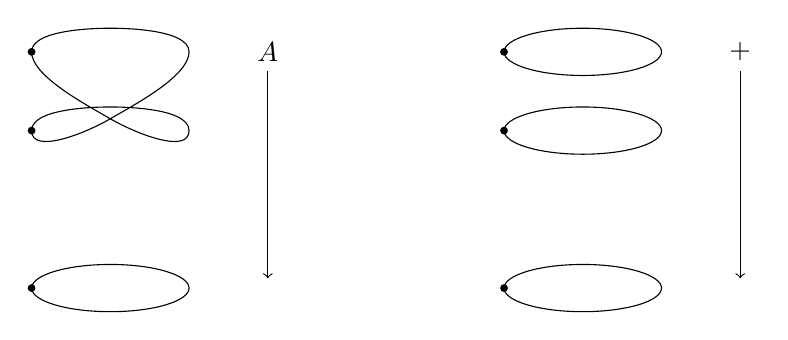
\begin{tikzpicture}
    \node (A) at (2,1) {$A$};
    \node (B) at (2,-2) {$\Sc$};
    \draw[->] (A) -- (B);
    \draw (0,-2) ellipse (1 and .3);
    \draw (-1,0)
    .. controls ++( 90:-.3) and ++(210: .4) .. (0,0.15)
    .. controls ++(210:-.4) and ++(270: .3) .. (1,1)
    .. controls ++(270:-.3) and ++(  0: .1) .. (0,1.3)
    .. controls ++(  0:-.1) and ++( 90: .3) .. (-1,1)
    .. controls ++( 90:-.3) and ++(150: .4) .. (0,0.15)
    .. controls ++(150:-.4) and ++(270: .3) .. (1,0)
    .. controls ++(270:-.3) and ++(  0: .1) .. (0,0.3)
    .. controls ++(  0:-.1) and ++( 90: .3) .. (-1,0);
    \node[fill,circle,inner sep=1pt] at (-1,-2) {};
    \node[fill,circle,inner sep=1pt] at (-1,0) {};
    \node[fill,circle,inner sep=1pt] at (-1,1) {};
%    \node (L) at (1,-3) {(left)};
    \begin{scope}[xshift=6cm]
    \node (At) at (2,1) {$\Sc+\Sc$};
    \node (Bt) at (2,-2) {$\Sc$};
    \draw[->] (At) -- (Bt);
    \draw (0,-2) ellipse (1 and .3);
    \draw (0,0) ellipse (1 and .3);
    \draw (0,1) ellipse (1 and .3);
    \node[fill,circle,inner sep=1pt] at (-1,-2) {};
    \node[fill,circle,inner sep=1pt] at (-1,0) {};
    \node[fill,circle,inner sep=1pt] at (-1,1) {};
%    \node (Lt) at (1,-3) {(right)};
    \end{scope}
  \end{tikzpicture}
  \end{sidecaption}
\end{figure}

\begin{xca}\label{xca:twoS1coverings}
In this exercise you are asked to elaborate the difference
between $A$ and $A'$ above.
Let $c_\bool \defeq (z\mapsto\bool): \Sc\to\Set$.
\begin{enumerate}
\item
This part is about $A'$. Show that $\sum_{z:\Sc}\bool$ is not connected.
Give an element of the type $c_\bool\eqto\ve_\Set(\bool,\refl{\bool})$.
\item
One can define $A$ by $A\defeq\sum_{z:\Sc}\ve_\Set(\bool,\twist)$.
Show that $A$ is connected.
Give an element of type $(c_\bool\eqto\ve_\Set(\bool,\twist))\to\false$.
Hint: use \cref{xca:C2} and \cref{lem:freeloopspace}.\qedhere
\end{enumerate}
\end{xca}

\begin{remark}
  It \emph{is} possible to misunderstand what a ``connected \covering'' is:
the other interpretation ``all the preimages are connected''
would simply give us an equivalence (since connected sets are contractible),
and this is \emph{not} what is intended. (Equivalences are \coverings,
but not necessarily connected \coverings and connected \coverings are not necessarily equivalences.)

Likewise for the other qualifications; for instance, in a ``finite \covering'' $f:A\to B$,
all fibers are finite sets, but 
the type $A$ is usually \emph{not} a finite set.

We trust the reader to keep our definitions in mind and not the other interpretations.
\end{remark}


\begin{remark}
  \Coverings are closely related to a concept from topology called ``covering spaces''
(or any variant of this concept, including Galois theory) and from algebra as locally constant sheaves (of sets).
Either way, the concept is useful because it singles out the (sub)symmetries.
\end{remark}

In this chapter, we focus on \coverings over the circle.
We start by refining the notion of diagram introduced in
\cref{rem:diagram}.

\begin{remark}\label{rem:subtype-diagram}
Consider the left diagram below, where $i_1, i_2$
are injections constituting $S$ as a subtype of $X$ and
$T$ as a subtype of $Y$, respectively (see \cref{def:subtype}).\footnote{%
To stress that a function is an injection we may decorate
the $\to$ in its type with a hook: $\hookrightarrow$.}
This diagram represents the identity type $f\circ i_1 \eqto i_2\circ g$.
Since $i_2$ is an injection, the type
$\sum_{g:S\to T} (f\circ i_1 \eqto i_2\circ g)$ is a proposition.\footnote{%
Use \cref{xca:prod-of-fibs} to see this.}
\[
\begin{tikzcd}
  X \ar[r,"f"]  & Y &&
  X \ar[r,"f"]  & Y                          \\
  S \ar[r,"g"] \ar[u,hookrightarrow,"i_1"]        & T \ar[u,hookrightarrow,"i_2"'] &&
  X_P \ar[r,dashed,"g"] \ar[u,hookrightarrow,"\fst"]     & Y_Q \ar[u,hookrightarrow,"\fst"']
\end{tikzcd}
\]
In the right diagram we depict the case
in which $S$ is given by a predicate $P: X\to\Prop$
and $T$ is given by a predicate $Q: Y\to\Prop$,
with the injections being first projections of the right type.
We can now apply the universal property of subtypes
\cref{xca:subtype-univ-prop} to $Y_Q$ with
$(f\circ\fst) : X_P \to Y$ and get that the three propositions
$\prod_{z:X_P} Q(f(\fst(z)))$ and
$\prod_{x:X}(P(x)\to Q(f(x)))$ and
$\sum_{g:X_P\to Y_Q} (f\circ\fst \eqto \fst\circ g)$
are logically equivalent. If these propositions hold,
we say that $f$ \emph{respects the subtypes} and
we may call the diagram a \emph{subtype diagram}.
\index{diagram!subtype}

If $q$ is a proof of $\prod_{x:X}(P(x)\to Q(f(x)))$,
then we can uniquely define the function $g: X_P\to Y_Q$, 
the one labelling the dashed arrow in the right diagram above,
by $(x,p) \mapsto (f(x),q(x,p))$. The functions $f\circ\fst$ and
$\fst\circ g$ are identified by reflexivity.
We may call $g$ the \emph{function induced by $f$ on subtypes},
and will also denote it by $f$.

Now consider the special case in which $f: X\to Y$ is an equivalence.
If the inverse of $f$ also respects the subtypes,
that is, if $\prod_{y:Y}(Q(y)\to P(\inv f(y)))$, then
the function that is induced by $f$ on the subtypes is
also an equivalence. Moreover, the functions induced by $f$ and $\inv f$
are then each other's inverses.
\end{remark}


\begin{theorem}\label{thm:coveringsofS1perms}
In the diagram below, the equivalence $f$ in the second row
is $\preim$ from \cref{lem:typefamiliesandfibrations}, and
the equivalence $g$ in the same row is defined by 
$g(S)\defeq (S(\base),\trp[\id_\UU]{S(\Sloop)})$ 
(\cref{lem:freeloopspace} applied with $A\defeq\UU$, 
and \cref{def:idtoeq}).
Along the vertical arrows we have maps that forget the
property that constitutes its domain as a subtype of the
codomain, all modest variations of the first projection.

The statement of the theorem is now that the diagram below
is the composite of subtype diagrams (see \cref{rem:subtype-diagram})
in which the induced functions $f$ and $g$ 
in the third row are equivalences as well.

\[
\begin{tikzcd}
  && \sum_{X:\UU}(X\to X) \\ %& \sum_{X:\UU}(X\to X\to\UU) 
  \bigl(\sum_{A:\UU}(A\to\Sc) \ar[r,equivr,"f"]\bigr) & 
  \bigl(\Sc\to\UU \ar[r,equivr,"g"]\bigr) & 
  \sum_{X:\UU}(X\equivto X) \ar[u,hookrightarrow]                         
\\
  \SetBundle(\Sc) \ar[r,equivl,"f"'] \ar[u,hookrightarrow]  &
  \bigl(\Sc\to\Set\bigr) \ar[r,equivl,"g"'] \ar[u,hookrightarrow]  &
  \sum_{X:\Set}(X\equivto X) \ar[u,hookrightarrow]
\end{tikzcd}
\]
\end{theorem}
\begin{proof}
We prove first that $\preim$ respects the subtypes. 
Let $A:\UU$ and $h: \Sc\to A$ such that $(A,h)$ is a \covering.
This means that $\inv h(a)$ is a set, for any $a:A$.
Since $\preim(A,h)(a) \jdeq \inv h(a)$, we immediately get
that $\preim(A,h) : \Sc\to\Set$. 
In order to prove that $\inv\preim$ also respects the subtypes
one simply reverses this argument.

Next we prove that $g$ respects the subtypes.
Let $S: \Sc\to\UU$ be such that $S(z)$ is a set for all $z:\Sc$.
This means in particular that $S(\base)$ is a set.
Since $g(S)\jdeq (S(\base),\trp{S(\Sloop)})$, we are done.
In order to prove that $\inv g$ also respects the subtypes
we reason as follows. Let $X:\UU$ and $h: X\equivto X$ be given.
Assume that $X$ is a set. We have $\inv g(X,h)\jdeq
\ve_\UU(X,\etop{h})$, see \cref{lem:freeloopspace}
and \cref{def:univalence}.
Now, since $X\jdeq\ve_\UU(X,\etop{h})(\base)$ is a set 
and $\Sc$ is connected,
we have $\inv g(X,h): \Sc\to\Set$ and we are done.

Note that the left subtype diagram is fully general:
it also holds when we replace $\Sc$ by any type $B$.
This is not true for the right subtype diagram.
\end{proof}

In slogan form: A \covering over the circle is a set with
a permutation of its elements.
The fiber over $\base:\Sc$ gives the set,
and transporting along $\Sloop$ gives the permutation.

\begin{example}\label{def:universalcover}
A simple yet important example of a \covering over a groupoid
$B$ with an element $b_0$ is given by the family of identity types 
$\uc{b_0}(b) \defeq (b_0 \eqto b)$ parameterized by $b:B$.
\glossary(universal){$\protect\uc{b_0}$}%
{the type family $b \mapsto (b_0 \protect\eqto b)$} 
These identity types are indeed sets since $B$ is a groupoid. 
The alternative form
of this (pointed) set bundle is the map $\fst: \sum_{b:B}(b_0\eqto b)\to B$,
the domain canonically pointed at $(b_0,\refl{b_0})$, and with 
$\refl{b_0}$ as the pointing path of $\fst$.

In the above example, the reader may have noticed that,
by \cref{lem:thepathspaceiscontractible}, 
$\sum_{b:B}(b_0\eqto b)$ is contractible. Hence yet another
form of this \covering is the constant map 
$\cst{b_0}:\bn{1}\to B$, also with pointing path $\refl{b_0}$.
%The alternative form of this \covering is given by the
%fibers of $\cst{b_0}$. By definition, 
%$\inv\cst{b_0}(b)\jdeq \sum_{i:\bn{1}} b\eqto b_0$,
%so that these fibers can be identified with $b_0\eqto b$ by univalence.
What is special about these examples is captured by the
following definition and ensuing lemma.
\end{example}

\begin{definition}\label{def:univ-cover}
Let $A$ and $B$ be pointed types and $f: A\ptdto B$ a pointed \covering.
We call $f$ \emph{universal} if for every pointed \covering $g: C\ptdto B$
there is a unique $h: A\ptdto C$ with $f\eqto gh$, that is, if
the following type is contractible:
\[\sum_{h: A\ptdto C} f\eqto_{A\ptdto B} gh.\qedhere\]
\end{definition}

In the above definition we get that $h: A\ptdto C$ is a
\covering as well by \cref{xca:covering-utils}\ref{it:left-cancel-cover}.
The examples preceding \cref{def:univ-cover} are indeed universal
\coverings according to the following lemma.

\begin{lemma}\label{lem:univ-cover-of-groupoid}
Let $(A,a_0)$ be a pointed type, $(B,b_0)$ a pointed
groupoid, and $f : (A,a_0)\ptdto (B,b_0)$ a pointed \covering. 
Then $f$ is universal if and only if $A$ is contractible. 
\end{lemma}

\begin{proof}
Let conditions be as above and assume $A$ is contractible.
Let $(C,c_0)$ be a pointed type and $g: (C,c_0)\ptdto (B,b_0)$
a \covering. Let $f_0 : b_0\eqto f(a_0)$ and $g_0 : b_0\eqto g(c_0)$
be the respective pointing paths. 
Define $h: (A,a_0)\ptdto (C,c_0)$ by $a\mapsto c_0$ with
pointing path $\refl{c_0}$.
Clearly $g_0\inv f_0 : f(a_0) \eqto g(h(a_0))\jdeq g(c_0)$,
which yields an identification of $f(a)$ and $g(h(a))$ for all $a:A$
as $A$ is contractible. Apply now function extensionality
\cref{def:funext} to get an identification of type $f \eqto_{A\to B} gh$.
The pointing path of $gh$ is also $g_0 : b_0 \eqto g(c_0)$.
We get an identification of type $(f,f_0)\eqto_{A\ptdto B} (gh,g_0)$
since $g_0 = (g_0\inv f_0) f_0$.%
\marginnote{Draw the triangle!}
The type $(A,a_0)\ptdto (C,c_0)$ is contractible since $A$ is
contractible, yielding that $h$ is unique. 

For the other direction of the lemma we use a reasoning pattern
that is typical for universality. Assume that $f$ is universal.
As shown above, $\cst{b_0}: \bn{1}\ptdto (B,b_0)$ is also universal.
Hence we have maps $h$ and $h'$ and identifications
of all identity types represented in the following diagram,
simplified by ignoring the points:  
  \[
    \begin{tikzcd}[column sep=large,ampersand replacement=\&]
      \bn 1\ar[rr,"h'"]\ar[drrr,"\cst{b_0}"'] \& \& 
      A \ar[rr,"h"] \ar[dr,pos=.7,"f"] \& \& 
      \bn 1\ar[rr,"h'"]\ar[dl,pos=.7,"\cst{b_0}"'] \& \& 
      A \ar[dlll,"f"]             \\
      \& \& \& B \& \& \& 
    \end{tikzcd}
  \]
Using the universality of $f$, we can identify $h'h$ with $\id_A$.
Using the universality of $\cst{b_0}$, we can identify $hh'$ with $\id_\bn{1}$.
Now \cref{lem:weq-iso} yields an equivalence between $\bn{1}$
and $A$, implying that $A$ is contractible.
\end{proof}

A particularly important example of a pointed \covering is the following.

\begin{definition}\label{def:RtoS1}
  Recall the set of integers $\zet$ from \cref{def:zet}, with
  its successor function $\zs: \zet\equivto\zet$ being an
  equivalence. The \covering $R:\Sc\to\UU$ is defined by
  the recursion principle of the circle from \cref{def:circle}
  by putting $R(\base)\defeq\zet$ and $R(\Sloop)\defis \etop{\zs}$.
  This is indeed a set bundle since $\Sc$ is connected,
  so that $R(x)$ is a set for all $x:\Sc$.
  We also write $R:\Sc\to\Set$.
  Recall $\Tot(R)\jdeq\sum_{z:\Sc}R(z)$ and point $\Tot(R)$ 
  at $(\base,0)$. Now define
  \[
    \exp\defeq\fst:\Tot(R) \to \Sc,
    \text{~with pointing path~}\refl{\base}.
  \]
  We call $\exp$ the \emph{exponential \covering over the circle}.
\end{definition}

\begin{remark} \label{rem:expforreal}%
  \begin{marginfigure}
    \begin{tikzpicture}[scale=.15]
      \node (Sc) at (0,-5) {$\Sc$};
      \node[dot,label=left:$2$]  (B)    at (-10,18) {};
      \node[dot,label=left:$1$]  (one)  at (-10,14) {};
      \node[dot,label=left:$0$]  (zero) at (-10,10) {};
      \node[dot,label=left:$-1$] (mone) at (-10, 6) {};
      \node[dot,label=left:$-2$] (C)    at (-10, 2) {};
      \node[dot]                 (D)    at (-10,-5) {};
      \node[label=above:$\Tot(R)$]   (R)    at (10,20) {};
      \node[label=above left:$\zet$]  (Z)    at (-10,20) {};
      \node at (-10,20.8) {$\vdots$};
      \node at (-10,.2) {$\vdots$};
      \node[label=left:$\Sloop$] (Sloop) at (10,-5) {};

      \pgfmathsetmacro\cc{.55228475}% = 4/3*tan(pi/8)
      \pgfmathsetmacro\cy{2*\cc}%
      \pgfmathsetmacro\cx{10*\cc}%
      \pgfmathsetmacro\ay{.35165954}%

      \draw (10,0) \foreach \y in {0,4,...,16} {
        .. controls (10,\y + \cy + \ay) and (\cx,3 + \y - \ay)
        .. (0,3 + \y) .. controls (-\cx,3 + \y + \ay) and (-10,2 + \y + \cy - \ay)
        .. (-10,2 + \y) .. controls (-10,2 + \y - \cy + \ay) and (-\cx,1 + \y - \ay)
        .. (0,1 + \y) .. controls (\cx,1 + \y + \ay) and (10,4 + \y - \cy - \ay)
        .. (10,4 + \y) } ;
      \draw (10,-5) .. controls (10,-5 + \cy) and (\cx,-3)
      .. (0,-3) .. controls (-\cx,-3) and (-10,-5 + \cy)
      .. (-10,-5) .. controls (-10,-5 - \cy) and (-\cx,-7)
      .. (0,-7) .. controls (\cx,-7) and (10,-5 - \cy) .. (10,-5);
    \end{tikzpicture}
  \end{marginfigure}
  The reason for the name ``exponential'' comes from the following
  visualization.  If $x$ is a real number, then the complex
  exponentiation $\ee^{2\pi\ii x}=\cos(2\pi x)+\ii\sin(2\pi x)$ has
  absolute value $1$ and so defines a continuous function
  to the unit circle $\setof{(x,y):\RR^2}{x^2+y^2=1}$,
  where we have identified $\RR^2$ with the complex numbers.
  Choosing any point $z$ on the unit
  circle, we see that the preimage of $z$ under the exponential
  function is a shifted copy of the integers inside the reals.\footnote{%
    \emph{homotopy types} have to wait until Appendix B.3}

  This connection between the integers and the unit circle is
  precisely captured in a form that we can take further by studying the
  \covering $\exp:\Tot(R)\to \Sc$.
\end{remark}

In the next section we will see that the exponential \covering
of the circle is in fact universal.
We'll continue the general study of \coverings in \cref{sec:gsets}
and indeed throughout the book.
For now, we'll focus our attention on the circle and \coverings over it.

\section{The symmetries in the circle}
\label{sec:symcirc}

With the set $\zet$ of integers \emph{defined} as in \cref{sec:integers},
we will now construct an equivalence between $\zet$ and the type
$\base\eqto_{\Sc}\base$, and that under this equivalence $0:\zet$ corresponds to
$\refl{\base}:\base\eqto \base$, and $1$ to $\Sloop$, and $-1$ to $\Sloop^{-1}$.
More generally, the successor $\zs:\zet\to\zet$ corresponds to composition  
with $\Sloop$, while the predecessor $\inv{\zs}$ corresponds to composition 
with $\Sloop^{-1}$.\marginnote{%
  It follows directly that \emph{addition} of integers corresponds
  to \emph{composition} of loops.}

The first step is to identify the exponential \covering \cref{def:RtoS1}
with the universal \covering in \cref{def:universalcover},
\ie identify the type family
\[
  R: \Sc\to\UU,\qquad R(\base)\defeq\zet,\, R(\Sloop)\defis \etop{\zs}
\]
with the family
\[
\uc{\base}:\Sc\to\UU,\qquad \uc{\base}(z)\defeq (\base\eqto z).
\]
What does it mean to identify the families $\uc{\base}$ and $R$?
Type families are a special case of functions.
Function extensionality reduces the question to the pointwise
identification of $\uc{\base}$ and $R$ as functions.
Using univalence, it suffices to give
an equivalence from $\uc{\base}(z)$ to $R(z)$ for every $z:\Sc$,
that is, recalling \cref{def:function-type-families}, giving
a (fiberwise) equivalence $f: \uc{\base}\to R$. We will use
\cref{lem:weq-iso}, so will also define $g: R\to\uc{\base}$.

\begin{remark}\label{rem:univalence-transparent}
We recall \cref{lem:trp-in-function-type} defining how
transport behaves in families of function types.
Given a type $A$ and two type families $P,Q:A\to\UU$,
transport along $p:a\eqto a'$ of $h:P(a)\to Q(a)$ can
be identified with the function
$\trp[Q]{p}\circ h\circ \trp[P]{p^{-1}}$
of type $P(a') \to Q(a')$. As a simplification we
could use the notation $\tilde{\blank}$ introduced
after \cref{def:univalence} for the transport functions.
However, we now take the further step of allowing
univalence to be completely transparent, 
that is, leaving out both $\tilde{\blank}$ and $\bar{\blank}$
when no confusion can occur. Here this means that
the picture for the transport of $h$ becomes:
\[
  \begin{tikzcd}[column sep=huge]
    a\ar[d,eqr,"p"] & P(a)\ar[r,"h"]\ar[d,equivr,"P(p)"] &
    Q(a)\ar[d,equivr,"Q(p)"] \\
    a' & P(a')\ar[r,"Q(p)\,h\,P(p)^{-1}"] & \,Q(a').
  \end{tikzcd}
\]
In, for example, the definition of the exponential
\covering $R$ above, this means that we may denote $R(\Sloop)$
as $\zs$ instead of $\etop{\zs}$, and may write $R(\Sloop)(0)=1$.
\end{remark} 

If $A$ is $\Sc$, then the induction principle for the circle says
that giving an $h(z):P(z)\to Q(z)$ for all $z:\Sc$ is the same as
specifying an element $h(\base):P(\base)\to Q(\base)$ and,
using \cref{def:pathover-trp} and \cref{rem:univalence-transparent},
an identification
$h(\Sloop):Q(\Sloop)\,h(\base)\,P(\Sloop)^{-1}\eqto h(\base)$,
see the following diagram:
\[
  \begin{tikzcd}[column sep=huge]
    P(\base)\ar[r,"h(\base)"]\ar[d,equivr,"P(\Sloop)"]
    & Q(\base)\ar[d,equivr,"Q(\Sloop)"] \\
    P(\base)\ar[r,"h(\base)"] & Q(\base).
  \end{tikzcd}
\]
If $P,Q$ are families of sets,
then $h(\Sloop)$ is a proof that this diagram commutes.

We now define $f: \uc{\base}\to R$ and $g: R\to\uc{\base}$ that will turn out to
give inverse equivalences between $\uc{\base}(z)$ and $R(z)$, for each $z:\Sc$.

\begin{marginfigure}
  \begin{tikzpicture}[scale=.15]
    \node (Sc) at (0,-5) {$\Sc$};
    \node[dot,label=above:$\vdots$] (B)    at (-10,18) {};
    \node[dot]                      (one)  at (-10,14) {};
    \node[dot]                      (zero) at (-10,10) {};
    \node[dot]                      (mone) at (-10, 6) {};
    \node[dot]                      (C)    at (-10, 2) {};
    \node[dot]                      (D)    at (-10,-5) {};
    \node[label=above:$\Tot(R)$]    (R)    at (10,20) {};
    \node[label=above left:$\zet$]  (Z)    at (-10,20) {};
    \node at (-10,.2) {$\vdots$};
    \node[label=left:$\Sloop$] (Sloop) at (10,-5) {};

    \pgfmathsetmacro\cc{.55228475}% = 4/3*tan(pi/8)
    \pgfmathsetmacro\cy{2*\cc}%
    \pgfmathsetmacro\cx{10*\cc}%
    \pgfmathsetmacro\ay{.35165954}%

    \draw (10,0) \foreach \y in {0,4,...,16} {
      .. controls (10,\y + \cy + \ay) and (\cx,3 + \y - \ay)
      .. (0,3 + \y) .. controls (-\cx,3 + \y + \ay) and (-10,2 + \y + \cy - \ay)
      .. (-10,2 + \y) .. controls (-10,2 + \y - \cy + \ay) and (-\cx,1 + \y - \ay)
      .. (0,1 + \y) .. controls (\cx,1 + \y + \ay) and (10,4 + \y - \cy - \ay)
      .. (10,4 + \y) } ;
    \draw (10,-5) .. controls (10,-5 + \cy) and (\cx,-3)
    .. (0,-3) .. controls (-\cx,-3) and (-10,-5 + \cy)
    .. (-10,-5) .. controls (-10,-5 - \cy) and (-\cx,-7)
    .. (0,-7) .. controls (\cx,-7) and (10,-5 - \cy) .. (10,-5);

    \draw[->, bend left, shorten <=2pt, shorten >=2pt] (zero) to
    node[left] {\scriptsize$R(\Sloop)$} (one);%
    \draw[->, bend right, shorten <=2pt, shorten >=2pt] (zero) to
    node[left] {\scriptsize$R(\inv\Sloop)$} (mone);%
    \draw[->, bend right, shorten <=2pt, shorten >=2pt, line
    width=2pt, white] (zero) to (B);%
    \draw[->, bend right, shorten <=2pt, shorten >=2pt] (zero) to
    node[right,rounded corners,fill=white,outer sep=5pt]
    {\scriptsize$R(\Sloop^2)$} (B);%
    \draw[->, bend left, shorten <=2pt, shorten >=2pt, white, line
    width=2pt] (zero) to (C);%
    \draw[->, bend left, shorten <=2pt, shorten >=2pt] (zero) to
    node[right,rounded corners,fill=white,outer sep=5pt]
    {\scriptsize$R(\Sloop^{-2})$} (C);
  \end{tikzpicture}
  \caption{Transport in the family $R$}\label{fig:transportalongloop}
\end{marginfigure}
\begin{definition}
  \label{def:fPtoR}
  The function $f:\prod_{z:\Sc}(\uc{\base}(z)\to R(z))$ is defined by
  $f(z)(p)\defequi R(p)(0)$.
\end{definition}
In Figure~\ref{fig:transportalongloop}, the function $f(\base)(p)$
above has been visualised for $p\jdeq{\Sloop^n}$, $n\jdeq-2,-1,0,1,2$.

\begin{lemma}\label{lem:windingnumber}
For $f$ as in \cref{def:fPtoR} we have $f(\base)(\Sloop^n)=n$ for all $n:\zet$.
\end{lemma}
\begin{proof}
First consider positive $n:\NN$ and apply induction. 
In the base case $n=0$ we have
$f(\base)(\Sloop^0)\jdeq f(\refl\base)\jdeq\trp[R]{\refl\base}(0) \jdeq 0$.
For $n\jdeq\zs(m)$ with $m:\NN$ we have
\begin{alignat*}2
  f(\base)(\Sloop^{\zs(m)})&\jdeq R(\Sloop^{\zs(m)})(0)&\qquad&\\
  &= R(\Sloop \Sloop^{m})(0)&&\\
  &= R(\Sloop)(R(\Sloop^m)(0))&&\text{since $\ap{}$ preserves composition}\\
  &\jdeq R(\Sloop)(f(\base)(\Sloop^{m}))&&\\
  &= \zs(f(\base)(\Sloop^{m})) = \zs(m)&&\text{by the induction hypothesis.}
\end{alignat*}
This completes the induction step for positive $n$.
For negative $n$ the proof is similar.
\end{proof}

In the definition of the second map,
take into account that $R(\base)\jdeq \zet$ and $\uc{\base}(\base) \jdeq (\base\eqto \base)$.

\begin{definition}\label{def:gRtoP}
The function $g:\prod_{z:\Sc}(R(z)\to \uc{\base}(z))$ is
defined by circle induction. We first define
\[
g(\base)\defeq \left(n \mapsto {\Sloop^n} \right) :\zet\to(\base\eqto \base).
\]
Then, using \cref{rem:univalence-transparent}, the type $g(\Sloop)$ should be
\[
\uc{\base}(\Sloop)\, g(\base)\,R(\Sloop)^{-1}\eqto g(\base).
\]
\marginnote{%
  The type of $g(\Sloop)$ can be expressed by this diagram:
  \[
    \begin{tikzcd}[row sep=large,column sep=huge,ampersand replacement=\&]
      \zet\ar[r,"n\mapsto\Sloop^n"]\ar[d,equivr,"\zs"] \&
      (\base\eqto \base)\ar[d,equivr,"p\mapsto\Sloop\cdot p"] \\
      \zet\ar[r,"n\mapsto\Sloop^n"] \& (\base\eqto \base).
    \end{tikzcd}
  \]
}%
By definition,
$R(\Sloop)$ is $\zs$. Using \cref{xca:trp-in-a/x=b/x}\ref{trp-in-a=x}
we can identify $\uc{\base}(\Sloop)$ with composition with $\Sloop$.
The element $g(\Sloop)$ is obtained by function extensionality and
a simple calculation, using the identification of
${\Sloop\,\Sloop^{n-1}}$ and $\Sloop^n$ for any $n:\zet$.
\end{definition}

\begin{theorem}
  \label{lem:univisexp}
For every $z:\Sc$, the functions $f(z)$ defined in \cref{def:fPtoR}
and $g(z)$ in \cref{def:gRtoP} are inverse equivalences between
$\uc{\base}(z)$ and $R(z)$.
\end{theorem}
\begin{proof}
We apply \cref{lem:weq-iso} and verify the two conditions.
  First, we need to give elements $H(z,p):g(z)(f(z)(p))\eqto p$
for all $z:\Sc$ and $p:\uc{\base}(z)\jdeq(\base\eqto z)$.
By induction on $p:\base\eqto z$ it suffices to set
$H(\base,\refl\base)\defeq\refl{\refl{\base}}$ since
$g(\base)(f(\base)(\refl{\base}))\jdeq g(\base)(0)\jdeq\refl{\base}$.

Secondly, we need to give elements $G(z)(n):f(z)(g(z)(n))=n$
for all $z:\Sc$ and $n: R(z)$.
By circle induction it suffices to define $G(\base)$ and $G(\Sloop)$,
but the type of $G(\base)$ is a proposition (as $\zet$ is a set),
so the information for $G(\Sloop)$ is redundant.
Hence, it suffices to show that
$f(\base)(g(\base)(n))\jdeq  f(\base)(\Sloop^n)= n$ for all $n:\zet$.
This follows from \cref{lem:windingnumber}.
\end{proof}

\begin{corollary}\label{cor:S1groupoid}
The circle $\Sc$ is a groupoid, and the function
\[
{\Sloop}^{-} : \zet\to(\base\eqto_{\Sc}\base)
\]
sending $n$ to $\Sloop^n$ is an equivalence.
\end{corollary}
\begin{proof}
For any $z:\Sc$, the type $\uc{\base}(z)\jdeq (\base\eqto_{\Sc}z)$ is a set
since $R(z)$ is a set and $f(z):\uc{\base}(z) \to R(z)$ an equivalence.
Since the circle is connected and being a set is a proposition, it follows
that $y\eqto_{\Sc}z$ is a set, for any $y,z:\Sc$. Hence $\Sc$ is a groupoid.
By \cref{def:gRtoP}, ${\Sloop}^{-}\jdeq g(\base)$ is an equivalence.
\end{proof}

Recall the definition of universal \covering from \cref{def:univ-cover}.
Now that we know that the circle is a groupoid we can harvest
the following results.

\begin{corollary}\label{cor:univ-covers-S1}
The \covering $\uc{\base}$ from \cref{def:universalcover} is universal.
The exponential \covering $\exp$ from \cref{def:RtoS1} is universal.
\end{corollary}
\begin{proof} By \cref{lem:univ-cover-of-groupoid} and \cref{lem:univisexp}.
\end{proof}


\begin{definition}\label{def:windingnumber}
The inverse equivalence $f(\base)$ of $g(\base)\jdeq{\Sloop}^{-}
\jdeq(n\mapsto \Sloop^n)$ is called the \emph{winding number function}
  $\wdg : (\base \eqto\base) \equivto \zet$.
  \glossary(windingnumber){$\protect\wdg$}{winding number function}
\end{definition}
The following lemma is a simple example of a technique called 
\emph{delooping}, which we will further elaborate in \cref{sec:delooping}.
\begin{lemma}\label{lem:S1-delooping}
Let $A$ be a connected type and $a:A$ an element.
Assume we have an equivalence $e:(\base\eqto\base) \to (a\eqto a)$
of symmetries such that $e(\refl{\base})\eqto\refl{a}$
and $e(p\cdot q)\eqto e(p)\cdot e(q)$, for all $p,q:(\base\eqto\base)$.
Then $\check e : \Sc\to A$ defined by circle recursion by setting
$\check e(\base)\defeq a$ and $\check e(\Sloop)\defis e(\Sloop)$
is an equivalence.
\end{lemma}
\begin{proof}
We have $\ap{\check e}\eqto e$ since they produce equal values when applied
to $\Sloop^n$, for all $n:\zet$. Now use that $A$ and $\Sc$ are connected and
apply \cref{cor:fib-vs-path}\ref{conn-fib-vs-path}.
\end{proof}

\begin{xca}\label{xca:general-winding}
  Generalizing~\cref{def:windingnumber}, of winding numbers, use
  circle induction to define, for any point $x:\Sc$ of the circle an
  equivalence, $\wdg_x : (x \eqto x) \we \zet$.  (You'll need
  commutativity of addition in $\zet$.)  Conclude from
  \cref{lem:S1-delooping} that we have equivalences
  $f_x : \Sc \we \Sc$ with $f_x(\base) \jdeq x$, for each
  $x:\Sc$.\footnote{%
    If we think of the circle as represented by the unit length
    complex numbers, then $f_x(y)$ corresponds to the usual product
    $xy$.  Alternatively, if we think of points on the circle as
    representing rotations of the unit circle in $\RR^2$, then $f_x(y)$
    corresponds to the composition of the rotations by $x$ and $y$.}
\end{xca}

\begin{xca}\label{xca:S1=S1-components}
Let $-\id_\Sc : \Sc\to\Sc$ be defined by $-\id_\Sc(\base)\defeq\base$
and $-\id_\Sc(\Sloop)\defis{\Sloop}^{-1}$. Show the $-\id_\Sc$
and $\id_\Sc$ are not in the same component of $\Sc\to\Sc$.
Prove the following proposition:
\[
\prod_{t:\Sc\equiv\Sc}{\Trunc{\id_\Sc\eqto t}\amalg \Trunc{-\id_\Sc\eqto t}}.\qedhere
\]
\end{xca}

\begin{xca}\label{xca:(S1->S1)_(f)-eqv-S1}
For any $f: \Sc\to\Sc$, give an equivalence
from $\Sc$ to $(\Sc\to\Sc)_{(f)}$, that is, from $\Sc$ to
the component of $\Sc\to\Sc$ at $f$.
Hint: use \cref{lem:S1-delooping}.
\end{xca}

We note in passing that combining the above two exercises
yields an equivalence from $(\Sc\eqto\Sc)$ to $(\Sc\amalg\Sc)$,
that is, a characterization of the symmetries \emph{of} the cycle
(in constrast to the title of this \cref{sec:symcirc}).


\section{A reinterpretation of the circle}\label{sec:S1isC}

In this section we return to the equivalences in \cref{thm:coveringsofS1perms}.
We'll use these to get a different perspective on the circle,
which highlights it as a type classifying very simple symmetries,
namely sets with permutations.
We have already seen one example in \cref{def:RtoS1},
namely the set $\zet$ of integers together with the successor 
$\zs: \zet\equivto\zet$, defining the exponential \covering $\exp$.
By \cref{cor:univ-covers-S1}, $\exp$ and its friends
$\uc\base:\Sc \to \Set$ and $\cst\base : \bn 1 \to \Sc$
are appearances of the universal \covering over the circle.

The importance of $\exp$ will become apparent when we eventually
explain that \emph{the circle is equivalent to the connected component of
  $(\zet,\zs)$ in the type $\sum_{X:\UU}(X\to X)$}.\footnote{%
  The elements of this connected component can be thought of as
  \emph{infinite cycles}:
  sets $X$ with a successor function $t:X \to X$
  such that $(X,t)$ can be merely identified with $(\zet,\zs)$.
  That is, $(X,t)$ looks exactly like $(\zet,\zs)$,
  but we don't know which element of $X$ is ``zero'':\\[1ex]
  \begin{tikzpicture}[node distance=10pt]
    \begin{scope}[every node/.style={dot}]
      \node (x1) {};
      \foreach \p/\n/\deg in {1/2/27, 2/3/54, 3/4/81, 4/5/108, 5/6/135,%
        6/7/162, 7/8/135, 8/9/108, 9/10/81, 10/11/54, 11/12/27} {
        \node (x\n) [at=(x\p.\deg), anchor=\deg+180, shift=(\deg:10pt)] {};
      }
    \end{scope}
    \node (x0) [left=of x1] {$\ldots$};
    \node (x13) [right=of x12] {$\ldots$};
    \begin{scope}[->,shorten <=1pt,shorten >=1pt]
      \foreach \p/\n in {0/1, 1/2, 2/3, 3/4, 4/5, 5/6,
        6/7, 7/8, 8/9, 9/10, 10/11, 11/12, 12/13} {
        \draw (x\p)--(x\n);
      }
    \end{scope}
  \end{tikzpicture}}

Recall from \cref{thm:coveringsofS1perms}
the equivalence 
\[
gf: \SetBundle(\Sc) \equivto \sum_{X:\Set}(X\equivto X).
\]
When restricting to corresponding connected components,
we get equivalences between these. 
So to understand the components of $\SetBundle(\Sc)$
it suffices to understand the components of
$\sum_{X:\Set}(X\equivto X)$, which correspond to
components of $\sum_{X:\UU}(X \to X)$ at pairs $(X,t)$,
where $X$ is a set with a permutation $t$.\footnote{%
Given a set $X$ with a permutation $t$, 
we may coerce and view $(X,t)$ as an element of $\sum_{X:\UU}(X\to X)$. 
Then, for any $(Y,u)$ in the same connected component of
$\sum_{X:\UU}(X\to X)$ as $(X,t)$, we have that $Y$ also
is a set and $u$ also a permutation of $Y$.
}

We are particularly interested in understanding the symmetries 
in these components, so before we prove that the circle is equivalent 
to the component containing $(\zet,\zs$), let us investigate the 
equalities in the type $\sum_{X:\UU}(X \to X)$ a bit further.

Define the type family $D$ by $D(X) \defeq (X\to X)$ for all $X:\UU$.
Recall that, given $X,Y:\UU$ and $t:X\to X$ and $u:Y\to Y$,
\cref{lem:isEq-pair=} and \cref{def:pathover-trp} give
an equivalence between the identity type $(X,t)\eqto (Y,u)$ and
type of pairs consisting of a $p:X\eqto Y$ and an identification
of type $\trp[D]{p}(t)\eqto u$. The transport on the left is precisely
the special case described after \cref{lem:trp-in-function-type}
(see diagram in the margin),
\marginnote[-3\baselineskip]{%
  \begin{tikzcd}[column sep=huge,ampersand replacement=\&]
    X\ar[d,eql,"p"'] \&[-25pt]
    X \ar[r,"t"]\ar[d,equivl,"\ptoe p"'] \& X \ar[d,equivr,"\ptoe p"] \\
    Y\&[-25pt]
    Y \ar[r,"{\trp[D]{p}(t)}"'] \& Y
  \end{tikzcd}}
so that the latter identity type
type is equivalent to $\ptoe p\circ t\circ \ptoe p^{-1} \eqto u$.
If $p\jdeq\etop e$ for an equivalence $e:X\equivto Y$,
this is equivalent to $e\circ t \eqto u\circ e$, or $e t \eqto u e$ for short.
In total, we have an equivalence between the identity type 
$(X,t)\eqto(Y,u)$ and the sum type (see diagram in the margin)
\marginnote[-3\baselineskip]{%
  \begin{tikzcd}[column sep=huge,ampersand replacement=\&]
    X\ar[d,equivl,"e"'] \&[-25pt]
    X \ar[r,"t"]\ar[d,equivl,"e"'] \& X \ar[d,equivr,"e"] \\
    Y\&[-25pt]
    Y \ar[r,"u"'] \& Y
  \end{tikzcd}}
\[
  \sum_{e: X\equivto Y} et \eqto_{X\to Y} ue.
\]
These types are sets whenever $X$ and $Y$ are, and then we
may write $et = ue$. 
\begin{marginfigure}
  \begin{tikzpicture}[node distance=10pt]
    \begin{scope}[every node/.style={dot}]
      \node (x1) {};
      \foreach \p/\n/\deg in {1/2/72, 2/3/54, 3/4/81, 4/5/108, 5/6/135,%
        6/7/162, 7/8/135, 8/9/108, 9/10/81, 10/11/54, 11/12/72} {
        \node (x\n) [at=(x\p.\deg), anchor=\deg+180, shift=(\deg:10pt)] {};
      }
      \node (y1) [at=(x1.east), anchor=180, shift=(192:50pt)] {};
      \foreach \p/\n in {1/2, 2/3, 3/4, 4/5, 5/6,%
        6/7, 7/8, 8/9, 9/10, 10/11, 11/12} {
        \node (y\n) [at=(y\p.north), anchor=south, shift=(90:10pt)] {};
      }
    \end{scope}
    \node (x0) [below=of x1] {$\vdots$};
    \node (y0) [below=of y1] {$\vdots$};
    \node (x13) [above=of x12] {$\vdots$};
    \node (y13) [above=of y12] {$\vdots$};
    \node (Xf)  [above=26pt of x12] {$(X,t)$};
    \node (Zs)  [left=2pt of y13] {$(\zet,\zs)$};
    \node (zero)  [left=2pt of y6] {$0$};
    \begin{scope}[->,shorten <=1pt,shorten >=1pt]
      \foreach \p/\n in {0/1, 1/2, 2/3, 3/4, 4/5, 5/6,
        6/7, 7/8, 8/9, 9/10, 10/11, 11/12, 12/13} {
        \draw (x\p)--(x\n);
        \draw (y\p)--(y\n);
      }
    \end{scope}
    \begin{scope}[casblue,<-,shorten <=1pt,shorten >=1pt]
      \foreach \n in {1,2,...,12} {
        \draw (x\n)--(y\n);
      }
    \end{scope}
  \end{tikzpicture}
  \caption{An identification of two infinite cycles.
    The equivalence $e : \zet \protect\equivto X$ is marked in blue.}\label{fig:Zs=Xt}
\end{marginfigure}
In particular, given a set $X$ with a permutation $t$,
we have an equivalence from $(\zet,\zs)\eqto(X,t)$ to
$\sum_{e:\zet\equivto X}e\zs=te$. See \cref{fig:Zs=Xt} for an illustration.
This equivalence is transparent in the sense that we never denote it.
For example, any power $\zs^n$ of $\zs$ itself gives a symmetry
$(\zs^n,p) : (\zet,\zs)\eqto(\zet,\zs)$, where $p$ is a proof of
$\zs^n \zs = \zs \zs^n$.

\begin{remark}\label{rem:bang}
The type $\zs^n \zs = \zs \zs^n$ in the paragraph above is a proposition.
Since all elements of a proposition are equal, it is often not necessary
to name such elements explicitly. If the proposition in question is clear
from the context, we may use $!$ as a default name of its elements.
\glossary(0a){$\protect\bang$}%
{placeholder for an element (proof) of a proposition}
Be warned that different occurrences of $!$ may refer to elements of 
different propositions. In cases where the element of a proposition is 
not of interest (beyond its mere existence), we may even just ignore it.
For example, again in the paragraph above, we may ignore $p$ and
consider $\zs^n$ as a symmetry of $(\zet,\zs)$.
(Note that we did already coerce the \emph{function} $\zs^n$ to
the \emph{equivalence}.)
\end{remark}

The following property jumps out at us when we contemplate~\cref{fig:Zs=Xt}:
the equivalence $e$ is uniquely determined by the element $e(0):X$.
More precisely:
\begin{lemma}
  \label{lem:IdCisZet}
For every $(X,t)$ in the component of $\sum_{X:\UU}(X\to X)$
containing $(\zet,\zs)$, the function
  \[
    \ev_0:\bigl((\zet,\zs)\eqto(X,t)\bigr)\to X
    \text{~~defined by~~} \ev_0(e,!) \defeq e(0)
  \]
  is an equivalence.
\end{lemma}
\begin{proof}
  We'll prove that every fiber of $\ev_0$ is contractible.
  Given $x_0:X$ we must determine a unique equivalence $e:\zet\to X$
  such that $es=te$ and $e(0)=x_0$.
  Induction on $n:\zet$ (positive and negative $n$ separately)
  shows that for such an $e$, we have $e(n) = t^n(x_0)$ for all $n:\zet$.
  It remains to prove that $n\mapsto t^n(x_0)$ is an equivalence,
  for every $x_0:\zet$. Since we are proving a proposition,
  and we are assuming $(X,t)$ is in the component of $(\zet,\zs)$,
  it suffices to prove it for $(X,t) \jdeq (\zet,\zs)$.
  Clearly, for any $x_0,n:\zet$, we have $\zs^n(x_0) = n + x_0$,
  and the map $n \mapsto n + x_0$ is an equivalence,
  with inverse $n \mapsto n - x_0$.
\end{proof}
In particular, $\ev_0: ((\zet,\zs)\eqto(\zet,\zs))\to \zet$ is an equivalence,
mapping $\zs^n$ to $n$ for all $n:\zet$. 
Cf.\ $\wdg : (\base\eqto\base)\to\zet$ from \cref{def:windingnumber}.

\begin{definition}\label{def:S1toC}
  Let $\InfCyc$ be the component of $\sum_{X:\UU}(X\to X)$ 
  containing $(\zet,\zs)$.
  \glossary(InfCyc){$\protect\InfCyc$}{the type of infinite cycles,
  \cref{def:S1toC}}\index{cycle!infinite}
  Elements of $\InfCyc$ are called \emph{infinite cycles}.\footnote{%
    See also~\cref{def:Cyc} below for general cycles.}

  Define by circle induction
  \[
    c:\Sc\to\InfCyc \text{~~setting~~}
    c(\base)\defequi (\zet,\zs)
  \]
  and $c(\Sloop): c(\base)\eqto c(\base)$ given by the 
  \emph{predecessor} equivalence $\zs^{-1}: (\zet\to\zet)$
  and the trivial proof of the proposition $\zs^{-1}\zs=\zs\zs^{-1}$.
\end{definition}
\begin{marginfigure}
  \noindent\begin{tikzpicture}[scale=.15]
    \node (Sc) at (0,-5) {$\Sc$};
    \node[dot]                 (D)    at (-10,-5) {};
    \node[label=above left:$\uc{\color{casred}\base}({\color{casblue}\base})$] (Z) at (-10,20) {};
    \node at (-10,24.8) {$\vdots$};
    \node at (-10,.2) {$\vdots$};
    \node[label=left:$\Sloop$] (Sloop) at (10,-5) {};

    \pgfmathsetmacro\cc{.55228475}% = 4/3*tan(pi/8)
    \pgfmathsetmacro\cy{2*\cc}%
    \pgfmathsetmacro\cx{10*\cc}%
    \pgfmathsetmacro\ay{.35165954}%

    \draw[dashed] (10,0)
    .. controls (10,\cy + \ay) and (\cx,3 - \ay)
    .. (0,3) .. controls (-\cx,3 + \ay) and (-10,2 + \cy - \ay)
    .. (-10,2);
    \foreach \y/\col in {0/dashed,4/casred,8/black,12/casblue,16/dashed} {
      \draw[\col] (-10,2 + \y)
      .. controls (-10,2 + \y - \cy + \ay) and (-\cx,1 + \y - \ay)
      .. (0,1 + \y) .. controls (\cx,1 + \y + \ay) and (10,4 + \y - \cy - \ay)
      .. (10,4 + \y) .. controls (10,4 + \y + \cy + \ay) and (\cx,7 + \y - \ay)
      .. (0,7 + \y) .. controls (-\cx,7 + \y + \ay) and (-10,6 + \y + \cy - \ay)
      .. (-10,6 + \y);
    }
    \draw[dashed] (-10,22)
    .. controls (-10,22 - \cy + \ay) and (-\cx,21 - \ay)
    .. (0,21) .. controls (\cx,21 + \ay) and (10,24 - \cy - \ay)
    .. (10,24);
    \foreach \y in {2,6,...,22} {
      \node[dot] (B\y) at (-10,\y) {};
    }
    \draw (10,-5) .. controls (10,-5 + \cy) and (\cx,-3)
    .. (0,-3) .. controls (-\cx,-3) and (-10,-5 + \cy)
    .. (-10,-5) .. controls (-10,-5 - \cy) and (-\cx,-7)
    .. (0,-7) .. controls (\cx,-7) and (10,-5 - \cy) .. (10,-5);
  \end{tikzpicture}
  \caption{For the fiber of the universal \covering,
    $\uc{\color{casred}\base}({\color{casblue}\base}) \jdeq
    ({\color{casred}\base} = {\color{casblue}\base})$,
    we \emph{increase} the winding number when we transport
    the endpoint (in blue) along $\Sloop$, and
    we \emph{decrease} it when we transport the starting point
    (in red) in the same way.}\label{fig:plus-minus-one}
\end{marginfigure}

As explained in \cref{rem:bang}, we often leave out the propositional
data pertaining to $\InfCyc$ (and other subtypes) from the notation.

The main result of this section is \cref{thm:S1bysymmetries} below,
stating that the function $c$ from \cref{def:S1toC} is an equivalence.
Since it's such a crucial result, we are going to give two proofs.
Each proof illuminates a different aspect and gives methods
that will be used later.

For the first, we return to the equivalences of \cref{thm:coveringsofS1perms}.
As said above, these restrict to equivalences between corresponding components.
In particular, $\ev_\UU : (\Sc \to \UU) \equivto
\sum_{X:\UU} (X\equivto X)$ maps the type family $\uc{\base}$ to the pair
$(\base\eqto  \base, {\Sloop}{\cdot}\blank)$,
which can be identified with $(\zet,\zs)$ through~\cref{cor:S1groupoid}.
Hence, $\ev_\UU$ restricts to an equivalence between the
connected component of $\uc\base$ in $\Sc \to \UU$ and the connected component
of $(\zet,\zs)$ in $\sum_{X:\UU}(X\equivto X)$.

Recall the constant maps $\cst z: (\bn 1\to\Sc)$ for $z:\Sc$.
The equivalence $\preim$ maps $\cst\base$ to
$(x:\Sc) \mapsto \sum_{\_:\bn 1}(x\eqto \base)$
which can be identified with $\uc\base$.
Now consider the following diagram:
\begin{equation}\label{eq:setbundle-Sc-univ-comp}
  \begin{tikzcd}
    & \Sc\ar[dl,"{(\bn 1,\cst{\blank})}"']\ar[d,"\uc{\blank}"]\ar[dr,"c"] & \\
    \conncomp{\SetBundle(\Sc)}{\bn1,\cst\base} \ar[r,equivl,"\preim"']
    & \conncomp{(\Sc\to\UU)}{\uc\base} \ar[r,equivl,"\ev_\UU"']
    & \InfCyc
  \end{tikzcd}
\end{equation}
%where the last row is indeed well defined.
Both the left and the right triangle represent identity types.
We have an identification for the left triangle
because the fiber $\sum_{\_:\bn 1}(x\eqto z)$ of $\cst z$ at $x:\Sc$ can be identified with $\uc{z}(x) \jdeq (z\eqto x)$, for any $z:\Sc$.
For the right triangle we apply circle induction to construct an element
of $\prod_{z:\Sc}c(z) \eqto \ev_\UU(\uc{z})$.
The base case $z\jdeq\base$ is exactly the abovementioned application
of \cref{cor:S1groupoid}. For the loop case
we observe that the following diagram commutes:
\[
  \begin{tikzcd}[row sep=large,column sep=huge]
    \zet\ar[r,"\Sloop^-"]\ar[d,"\inv{\zs}"] &
    (\base\eqto \base)\ar[d,"\blank\cdot\Sloop^{-1}"] \\
    \zet\ar[r,"\Sloop^-"] & (\base\eqto \base).
  \end{tikzcd}
\]
Note that to transport in the family $\uc{-}(\base) \jdeq (\blank\eqto\base)$,
we use \cref{xca:trp-in-a/x=b/x}\ref{trp-in-x=a},
and \emph{that} is why we picked the predecessor equivalence in~\cref{def:S1toC}.
This is also illustrated in \cref{fig:plus-minus-one}.\footnote{%
  Another option would have been to choose the opposite equivalence $\zet\equivto\uc\base(\base)$, sending $n$ to $\Sloop^{-n}$, in the base case.
  The point is: You can move the minus sign around, but it has to pop up somewhere.}

With~\eqref{eq:setbundle-Sc-univ-comp} in hand, we see that $c$ is an equivalence
if and only if either of the two other downward maps are.\footnote{%
  At this point we could conclude with an appeal to the type theoretic 
  Yoneda lemma, which states that the map $X \to (X \to \UU)$,
  sending $x$ to the family $y \mapsto (x\eqto y)$,
  is an injection for any type $X$.
  See \footnotemark{} for the Yoneda lemma in category theory.
  You are asked to prove the type theoretic variant in
  \cref{xca:TTYoneda}.}\footcitetext{RiehlContext}
  
We now show that the map $(\bn 1,\cst{\blank})$ 
on the left is an equivalence. Since the codomain is connected,
it suffices to show that the fiber at $(\bn 1,\cst{\base})$ is contractible. 
This fiber is the sum type $\sum_{z:\Sc}((\bn 1,\cst \base)\eqto(\bn 1,\cst z))$,
where the identity type is by \cref{lem:isEq-pair=} equivalent to pairs of 
an equivalence $e : \bn 1 \to \bn 1$ and elements of the identity type
represented by the triangle
\[
  \begin{tikzcd}
    \bn 1 \ar[rr,"e"]\ar[dr,"\cst \base"'] & & \bn 1\ar[dl,"\cst z"] \\
    & \Sc. &
  \end{tikzcd}
\]
Since $\bn 1$ is contractible, this just amounts to the identity type
$\base\eqto z$, and $\sum_{z:\Sc}(\base\eqto z)$ is indeed contractible.

\begin{xca}\label{xca:TTYoneda}
Let $X$ be a type and $F: X\to\UU$ a function. Give an equivalence
$e_x$ from the identity type $(y \mapsto (x\eqto y)) \eqto F$
to the type $F(x)$, for any $x:X$. Then show that the map sending
$x:X$ to $(y \mapsto (x\eqto y)) : X\to\UU$
is an injection.
\end{xca}

We now give the second, more direct, proof that $c$ is an equivalence.
For this we use the following lemma, which is of independent interest.
\begin{lemma}\label{lem:conn-eq-f-ap-f-x}
Let $X$ and $Y$ be connected types, $x$ an element of $X$,
and $f$ a function from $X$ to $Y$. Then $f$ is an equivalence
if and only if $\ap{f}: (x\eqto x) \to (f(x)\eqto f(x))$ is an equivalence.
\end{lemma}
\begin{proof}
Using \cref{cor:fib-vs-path}\ref{conn-fib-vs-path} it suffices to show that
each map induced by $f$ on identity types is an equivalence if and only if the specific map
$\ap f : (x=x) \to (f(x) = f(x))$ is an equivalence.  Being an equivalence is a proposition,
so the result follows in two easy steps from $X$ being connected,
using \cref{xca:component-connected}.
\end{proof}

\begin{theorem}\label{thm:S1bysymmetries}
  The function $c:\Sc\to\InfCyc$ from \cref{def:S1toC} is an equivalence.
\end{theorem}
\begin{proof}
  In view of \cref{lem:conn-eq-f-ap-f-x} we only need to show that
$\ap{c}:(\base\eqto\base)\to((\zet,\zs)\eqto(\zet,\zs))$ is an equivalence.
Note that both the domain and the co-domain of $\ap{c}$ 
have been identified with $\zet$.
Consider the following diagram in which we compose $c$ with the equivalences
from \cref{cor:S1groupoid} and \cref{lem:IdCisZet}:
\[
  \begin{tikzcd}[column sep=large]
    \zet\ar[r,"\Sloop^-"] &
    (\base\eqto \base)\ar[r,"\ap{c}"] &
    \bigl((\zet,\zs)\eqto(\zet,\zs)\bigr)\ar[r,"\ev_0\vphantom{\ap{c}}"] &
    \zet
  \end{tikzcd}
\]
For $c$ to be an equivalence, it suffices to show that the composition
is an equivalence from $\zet$ to itself.
By definition, $\ap{c}(\Sloop)$ is the identification
corresponding to $\inv\zs$, sending $0$ to $-1$,
and by induction on $n:\zet$ it follows that
$\ev_0(\ap{c}(\Sloop^n)) = \zs^{-n}(0) = -n$.
And the map $n \mapsto -n$ is indeed an equivalence.
\end{proof}

\section{Connected \coverings over the circle}
\label{sec:covS1}

Let $A$ be a type and $f:A\to \Sc$ a function.
By \cref{cor:fib-vs-path}\ref{set-fib-vs-path}, $f$ is a \covering
over $\Sc$ if and only if each map induced by $f$ on identity types is injective.
Assume that $f:A\to \Sc$ is a \covering with $A$ connected.\marginnote{%
By \cref{xca:covering-utils}\ref{it:cover-n-type} $A$ is a groupoid.}
Let $a_0$ be an element of $A$. By \cref{xca:component-connected}
the condition that \emph{each} $\ap{f}$ is injective can be relaxed 
to $\ap{f}: (a_0\eqto a_0)\to(f(a_0)\eqto f(a_0))$ being injective.
Now look at the following diagram, with $\wdg$ the winding number
function from \cref{xca:general-winding} and ${\Sloop}^{-}$
from \cref{cor:S1groupoid}:

\begin{equation}\label{eq:subgroup-covering-1}
  \begin{tikzcd}
    (a_0 \eqto_A a_0) \ar[r,hookrightarrow,"{\ap{f}}"'] &
    (f(a_0)\eqto_\Sc f(a_0)) \ar[r,equivl,"{\wdg_{f(a_0)}}"'] &
    \zet \ar[r,equivl,"{{\Sloop}^{-}}"'] & (\base\eqto\base)
  \end{tikzcd}
\end{equation}
Define the composite $g_f\defeq\wdg_{f(a_0)}\circ\ap{f}$,
and consider its image, which is a subset of the integers.\marginnote{%
Since $A$ is connected, the proposition $\inv g_f(n)$ does not
depend on the choice of $a_0$, so the subset only depends on $f$.}
Clearly, $g_f$ is an injection, so that its fibers are propositions,
and the image is the subset $\sum_{n:\zet} \inv g_f(n)$.
Obviously, a classification of connected \coverings over the circle
also classifies certain subsets of $\zet$, or, equivalently,
certain subsets of symmetries of $\base$.\marginnote{%
  For subgroups in general, in \cref{ch:subgroups},
  the setbundle $f$ is pointed, 
  and has a pointing path $p: \pt_B \eqto f(\pt_A)$. Then
  $\ap{f}$ is composed with $\inv p \blank\, p$, conjugation.
  See also \cref{def:loops-map}.}
Such subsets of $\zet$ are closed under addition and negation,
and those of $(\base\eqto\base)$ are closed under concatenation and inverses,
since $\ap{f}$, $\wdg$ and ${\Sloop}^{-}$ are compatible with these operations.
Using language to be introduced in \cref{ch:subgroups}, 
we actually ``classify the subgroups of the integers''.

Recall that \coverings over the circle are equivalent to sets with permutations.
Which sets with permutations $(X,t)$ correspond to connected \coverings?
It is not so surprising that the answer has to do with whether
any two points $x,x':X$ can be connected by applying $t$ some number of times.

\begin{definition}\label{def:connected-by-t}
Let $X$ be a set with a permutation $t$. 
Elements $x,x':X$ such that $x'=t^n(x)$ for some $n:\zet$
are said to be \emph{connected} by $t$, denoted $x\sim x'$ 
whenever $t$ is clear from the context.\marginnote{%
    Recall that the iteration $t^n$ makes sense for all integers $n$
    since $t$ is an equivalence.}
    The relation $\sim$ is an equivalence relation.
    (Exercise: Check this.)
\end{definition}

Recall \cref{fig:covering}. We now have all the tools to
analyze the difference between the left and the right picture
in full generality.

\begin{construction}\label{con:cycset-connS1cover}
Let $X$ be a set with a permutation $t$, defining the equivalence
relation $\sim$ as in \cref{def:connected-by-t}.
The \covering over the circle corresponding to $(X,t)$ in
\cref{thm:coveringsofS1perms} is the pair $(\sum_{z:\Sc} E(z),\fst)$
where $E\defeq\ve_\UU(X,\etop{t}) : \Sc\to\UU$, with $\ve$ defined by
circle induction in \cref{lem:freeloopspace}.
Then we have a bijection between $\setTrunc{\sum_{z:\Sc} E(z)}$ and 
the quotient $X/\sim$ as defined in \cref{def:quotient-set}.
\end{construction}
\begin{implementation}{con:cycset-connS1cover}
Abbreviate $\sum_{z:\Sc} E(z)$ by $A$. We define a map
$g : \setTrunc A \to X/\sim$, from the set of components of $A$
to the quotient set of $X$ using the universal property of set 
truncation (\cref{def:set-truncation}), pair induction, and circle induction.
To define $g_0 : \prod_{z:\Sc}(E(z) \to X/\sim)$, we put
$g_0(\base)\defeq[\blank] : X \to X/\sim$ and need
$g_0(\Sloop) : \pathover{g_0(\base)}{E(\blank) \to X/\sim}{\Sloop}{g_0(\base)}$,
equivalent to $g_0(\base) \eqto_{X \to X/\sim} g_0(\base)t$.
The latter we get by function extensionality and \cref{thm:quotient-property},
since $x \sim t(x)$ for any $x:X$.

  The inverse of $h:(X/\sim) \to \setTrunc A$ of $g$
  is defined as the extension of $h_0 : X \to \setTrunc A$
  with $h_0(x) \defeq \settrunc{(\base,x)}$.
  We just need to check that $h_0(x) = h_0(x')$, or equivalently,
  $\Trunc{(\base,x)\eqto_A(\base,x')}$, whenever $x\sim x'$.
  Since this is a proposition, if $x'=t^n(x)$ with $n:\zet$,
  we may use induction on $n$ (positive and negative)
  together with the paths,
  $\pathpair{\Sloop}{\refl{t(x)}} : (\base,x)\eqto_A(\base,t(x))$,
  to conclude.

  It's easy to check that $g$ and $h$ are mutually inverse.
\end{implementation}

In \cref{fig:two-comp-S1-cover} we see the \covering corresponding
to the set $\set{1,2,3,4,5}$ with the permutation $1\mapsto 2\mapsto 3\mapsto 1,4\mapsto 5\mapsto 4$. There are two components, showing that the permutation splits into two cycles.
\begin{marginfigure}
  \begin{tikzpicture}[scale=.15]
    \node (Sc) at (0,-5) {$\Sc$};
    \node[dot,label=left:$5$] (four)  at (-10,22) {};
    \node[dot,label=left:$4$] (three) at (-10,18) {};
    \node[dot,label=left:$3$] (two)   at (-10,10) {};
    \node[dot,label=left:$2$] (one)   at (-10, 6) {};
    \node[dot,label=left:$1$] (zero)  at (-10, 2) {};
    \node[dot]                (D)     at (-10,-5) {};
    \node[label=left:$\Sloop$] (Sloop) at (10,-5) {};

    \pgfmathsetmacro\cc{.55228475}% = 4/3*tan(pi/8)
    \pgfmathsetmacro\cy{2*\cc}%
    \pgfmathsetmacro\cx{10*\cc}%
    \pgfmathsetmacro\intx{3.5}%
    \pgfmathsetmacro\inty{1.5}%
    \pgfmathsetmacro\ay{.35165954}%

    \draw (-10,18) .. controls (-10,18 - \cy + \ay) and (-\cx,17 - \ay)
    .. (0,17) .. controls (\cx,17 + \ay) and (10,20 - \cy - \ay) .. (10,20)
    .. controls (10,20 + \cy + \ay) and (\cx,23 - \ay)
    .. (0,23) .. controls (-\cx,23 + \ay) and (-10,22 + \cy - \ay)
    .. (-10,22) .. controls (-10,22 - \cy + \ay) and (-\cx,21 - \ay)
    .. (0,21) .. controls (\cx,21 + \ay) and (10,24 - \cy - \ay)
    .. (10,24)
    .. controls (10,24 + \cc) and (\intx + \cx, 24 + \inty + \ay)
    .. (\intx,24 + \inty) .. controls (\intx - \cx,24 + \inty - \ay)
    and (-\intx + \cx,20 + \ay)
    .. (-\intx,18 + \inty) .. controls (-\intx - \cx,18 + \inty - \ay)
    and (-10,18 + \cc) .. (-10,18);
    \draw (-10,2) .. controls (-10,2 - \cy + \ay) and (-\cx,1 - \ay)
    .. (0,1) .. controls (\cx,1 + \ay) and (10,4 - \cy - \ay)
    .. (10,4)
    \foreach \y in {4,8} {
      .. controls (10,\y + \cy + \ay) and (\cx,3 + \y - \ay)
      .. (0,3 + \y) .. controls (-\cx,3 + \y + \ay) and (-10,2 + \y + \cy - \ay)
      .. (-10,2 + \y) .. controls (-10,2 + \y - \cy + \ay) and (-\cx,1 + \y - \ay)
      .. (0,1 + \y) .. controls (\cx,1 + \y + \ay) and (10,4 + \y - \cy - \ay)
      .. (10,4 + \y) }
    .. controls (10,12 + \cc) and (\intx + \cx, 12 + \inty + \ay)
    .. (\intx,12 + \inty) .. controls (\intx - \cx,12 + \inty - \ay)
    and (-\intx + \cx,4 + \ay)
    .. (-\intx,2 + \inty) .. controls (-\intx - \cx,2 + \inty - \ay)
    and (-10,2 + \cc) .. (-10,2);
    \draw (10,-5) .. controls (10,-5 + \cy) and (\cx,-3)
    .. (0,-3) .. controls (-\cx,-3) and (-10,-5 + \cy)
    .. (-10,-5) .. controls (-10,-5 - \cy) and (-\cx,-7)
    .. (0,-7) .. controls (\cx,-7) and (10,-5 - \cy) .. (10,-5);
  \end{tikzpicture}
  \caption{A \covering with two components.}
  \label{fig:two-comp-S1-cover}
\end{marginfigure}

\begin{definition}\label{def:Cyc}
  Let $\Cyc$ be the subtype of $\sum_{X:\UU}(X\to X)$ of those
  pairs $(X,t)$ where $X$ is a \emph{\nonempty} set with an 
  \emph{equivalence} $t$ and any $x,x':X$ are connected by $t$.
  Expressed in a formula: \glossary(Cyc){$\protect\Cyc$}%
  {the type of cycles, \cref{def:Cyc}} \index{cycle}
\[
\Cyc \defeq \sum_{X:\Set}\bigl( {\Trunc X} \times \sum_{t:X\equivto X}
            \prod_{x,x':X}\exists_{n:\zet}(x'=t^n(x))\bigr).
\]
  Elements of $\Cyc$ are called \emph{cycles}.\footnote{%
    Our cycles are a special case of what is elsewhere called
    \emph{cyclically ordered sets},
    and they are closely related to the \emph{cyclic sets} of
    \citeauthor{Connes1983}\footnotemark{}.}\footcitetext{Connes1983}
\end{definition}
\begin{corollary}\label{thm:cycset-connS1cover}
  Under the equivalence described in \cref{con:cycset-connS1cover},
  connected \coverings over the circle correspond to cycles.
\end{corollary}
\begin{proof}
  We use the notations of the implementation of \cref{con:cycset-connS1cover}.
  If $A$ is connected, then $\setTrunc A$ is contractible and hence also
  $X/\sim$ is contractible, so $(X,t)$ is a cycle.
  
  Conversely, if $(X,t)$ is a cycle, then $X/\sim$ is contractible
  and hence also $\setTrunc A$ is contractible, so $A$ is connected. 
\end{proof}
  
We already know some connected \coverings over the circle, 
namely the universal \covering, which is also represented by 
the constant map $\cst\base:\bn 1\to\Sc$, and which we showed 
is equal to the exponential \covering, which in turn corresponds 
to the infinite cycle $(\zet,\zs)$
consisting of the set of integers $\zet$ with the successor permutation.
Another example is the left one of the two examples given in
\cref{fig:covering}.

We now introduce the remaining \coverings over the circle, first as functions to the circle, then as families of sets.
Eventually we'll show -- assuming a weak form
of the Law of the Excluded Middle -- that these (with the universal \covering)
are all the decidable connected \coverings over the circle.

\begin{definition}\label{def:mfoldS1cover}\index{degree!function}\index{function!degree $m$}
For $m:\NN$ positive, define the \emph{degree $m$ function} by circle induction
\[
\dg{m}:\Sc\to \Sc, \text{~~setting~}
\dg{m}(\base)\defeq\base \text{~~and~}
\dg{m}(\Sloop)\defis{\Sloop}^m.\qedhere
\]
\end{definition}
On loops, the degree $m$ function is the map
$(\blank)^m : (\base\eqto \base) \to (\base\eqto \base)$,\marginnote{%
Note that $(\blank)^0 : (\base\eqto \base) \to (\base\eqto \base)$
is constant and hence not injective.}
which is indeed an injection for positive $m$,
so $\dg{m}$ is a \covering corresponding to the subset of $(\base\eqto \base)$ consisting
of ${\Sloop}^{mn} : \base\eqto \base$ for all $n:\zet$.\marginnote{As a subset of $\zet$, this is simply all multiples of $m$.}

In~\cref{sec:symcirc} we gained a lot of insight into
the universal \covering, $\cst\base:\bn 1\to\Sc$,
by constructing an equivalence with the exponential \covering,
see \cref{lem:univisexp}.
In this section, we'll learn more about the degree $m$ map,
$\dg{m}:\Sc\to\Sc$,
by constructing an equivalence with another concrete family.

Fix a positive number $m:\NN$. Recall the finite set $\bn m$
from~\cref{def:finiteset} with elements denoted $0,1,\dots,m-1$,
as well as the equivalence of type $\bn m \equivto \sum_{k:\NN}k<m$
from \cref{xca:finite-types}.
Hence we may define a successor map $\zs : \bn m \to \bn m$ by
\[
  \zs(k) \defeq
  \begin{cases}
    k+1 & \text{if $k<m-1$,} \\
    0   & \text{if $k=m-1$.}
  \end{cases}
\]
\begin{exercise}
  Show that $\zs : \bn m \to \bn m$ is an equivalence by defining
  an explicit inverse.
\end{exercise}
Thus, $(\bn m,\zs)$ is another key example of a cycle called
the \emph{standard finite $m$-element cycle}.
As seen in \cref{thm:coveringsofS1perms},
any cycle corresponds to a \covering over $\Sc$.
Just as the \covering $R$ in \cref{def:RtoS1} corresponds to
the standard infinite cycle $(\zet,\zs)$,
we will now define the \covering $R_m$ corresponding to
standard finite $m$-element cycle.

\begin{definition}\label{def:RmtoS1}
  Fix $m:\NN$ positive. Define the \covering $R_m : \Sc\to\Set$ 
  by $R_m(\base) \defeq \bn m$ and
  $R_m(\Sloop) \defis \etop\zs$.  Recall
  $\Tot(R_m)\jdeq\sum_{z:\Sc}R_m(z)$ and point $\Tot(R_m)$ 
  at $(\base,0)$. Now define
  \[
    \pow{m} \defeq \fst : \Tot(R_m) \to \Sc \text{~with pointing path~}\refl{\base}.
  \]
We call $\pow{m}$ the \emph{$m$\th power bundle of the circle}.
  
\end{definition}
\begin{remark}\label{rem:finitecoveringsofS1}
  \begin{marginfigure}
    \begin{tikzpicture}[scale=.15]
      \node (Sc) at (0,-5) {$\Sc$};
      \node[dot,label=left:$4$] (four)  at (-10,18) {};
      \node[dot,label=left:$3$] (three) at (-10,14) {};
      \node[dot,label=left:$2$] (two)   at (-10,10) {};
      \node[dot,label=left:$1$] (one)   at (-10, 6) {};
      \node[dot,label=left:$0$] (zero)  at (-10, 2) {};
      \node[dot]                (D)     at (-10,-5) {};
      \node[label=above:$\Tot(R_m)$] (R) at  (0,20) {};
      \node[label=above left:$\bn m$] (m) at (-10,20) {};
      \node[label=left:$\Sloop$] (Sloop) at (10,-5) {};

      \pgfmathsetmacro\cc{.55228475}% = 4/3*tan(pi/8)
      \pgfmathsetmacro\cy{2*\cc}%
      \pgfmathsetmacro\cx{10*\cc}%
      \pgfmathsetmacro\intx{3.5}%
      \pgfmathsetmacro\inty{1.5}%
      \pgfmathsetmacro\ay{.35165954}%

      \draw (-10,2) .. controls (-10,2 - \cy + \ay) and (-\cx,1 - \ay)
      .. (0,1) .. controls (\cx,1 + \ay) and (10,4 - \cy - \ay)
      .. (10,4)
      \foreach \y in {4,8,12,16} {
        .. controls (10,\y + \cy + \ay) and (\cx,3 + \y - \ay)
        .. (0,3 + \y) .. controls (-\cx,3 + \y + \ay) and (-10,2 + \y + \cy - \ay)
        .. (-10,2 + \y) .. controls (-10,2 + \y - \cy + \ay) and (-\cx,1 + \y - \ay)
        .. (0,1 + \y) .. controls (\cx,1 + \y + \ay) and (10,4 + \y - \cy - \ay)
        .. (10,4 + \y) }
      .. controls (10,20 + \cc) and (\intx + \cx, 20 + \inty + \ay)
      .. (\intx,20 + \inty) .. controls (\intx - \cx,20 + \inty - \ay)
      and (-\intx + \cx,4 + \ay)
      .. (-\intx,2 + \inty) .. controls (-\intx - \cx,2 + \inty - \ay)
      and (-10,2 + \cc) .. (-10,2);
      \draw (10,-5) .. controls (10,-5 + \cy) and (\cx,-3)
      .. (0,-3) .. controls (-\cx,-3) and (-10,-5 + \cy)
      .. (-10,-5) .. controls (-10,-5 - \cy) and (-\cx,-7)
      .. (0,-7) .. controls (\cx,-7) and (10,-5 - \cy) .. (10,-5);
    \end{tikzpicture}
    \caption{The $m$\th power bundle for $m=5$.}
    \label{fig:m-th-power}
  \end{marginfigure}
  The analogue of our degree $m$ function is the $m$\th power of complex numbers
  restricted to the unit circle, mapping $z$ to $z^m$ if $|z|=1$.
  If we parameterize the unit circle by the angle $\theta:\RR$
  (defined up to multiples of $2\pi$),
  so $z=\ee^{\theta\ii}$, then $z^m = \ee^{m\theta\ii}$.
  \Cref{fig:m-th-power} illustrates the $m$\th power bundle over the circle.
  Choosing any point $z$ on the unit circle,
  we see that the preimage of $z$ under the $m$\th power map
  is a shifted copy of the $m$ different $m$\th roots of unity inside the unit circle.
\end{remark}
To identify $\dg{m}$ and $\pow{m}$ as \coverings over $\Sc$,
it suffices to define an equivalence $\psi_m : \Tot(R_m) \to \Sc$
and an identification $\alpha_m$ of the identity
type $\dg{m}\psi_m \eqto \pow{m}$ represented by the triangle below.
\[
  \begin{tikzcd}[column sep=small,ampersand replacement=\&]
    \Tot(R_m) \ar[rr,"\psi_m"]\ar[dr,"\pow{m}"'] \& \& \Sc\ar[dl,"\dg{m}"] \\
    \& \Sc \&
  \end{tikzcd}
\]

To see how to define $\psi_m$ and $\alpha_m$,
we draw in~\cref{fig:m-power-clock} the type $\Tot(R_m)$
unrolled into a ``clock'', with marks $0,1,\dots,m-1$
(the mark $k$ is the element $(\base,k):\Tot(R_m)$),
and arcs following the successor permutation of $\bn m$.
We denote these arcs by 
$a_k \defeq \pathpair{\Sloop}{\refl{\zs(k)}} : (\base,k) \eqto (\base,\zs(k))$.
The $m$\th power map (which is just the first projection)
sends each mark to $\base:\Sc$ and each arc to $\Sloop$.
\begin{marginfigure}
  \begin{tikzpicture}
    \foreach \n/\deg in {0/0, 1/72, 2/144, 3/216, 4/288} {
      \node[dot] (x\n) at (\deg:1) {};
      \node (l\n) [at=(x\n.\deg), anchor=\deg+180, shift=(\deg:2pt)] {$\n$};
      \draw[->,shorten <=1pt,shorten >=1pt] (x\n) arc (\deg:\deg+72:1);
      \node (p\n) at (\deg+36:.7) {$\color{casblue}{\Sloop}$};
    }
    \foreach \n/\deg in {0/0, 1/72, 2/144, 3/216} {
      \node (r\n) [at=(\deg+36:1), anchor=\deg+180]
      {\scriptsize$\color{casred}{\refl\base}$};
    }
    \node (r4) at (-36:1.3) {$\color{casred}{\Sloop}$};
  \end{tikzpicture}
  \caption{Unrolling $\protect\Tot(R_5)$ as a ``clock''. (Here we're going around in a counterclockwise fashion as mathematicians are wont to do.)}
  \label{fig:m-power-clock}
\end{marginfigure}
This is indicated in blue on the inside of the clock.
To define $\psi_m$, we must send all the marks to $\base:\Sc$
and all arcs to $\refl\base$, except one, which goes to $\Sloop$.
This is indicated in red on the outside of the clock.
\begin{construction}\label{con:psi-alpha-m}
  For each positive integer $m$,
  there is an equivalence $\psi_m : \Tot(R_m) \to \Sc$
  and an element $\alpha_m : \dg{m}\psi_m \eqto \pow{m}$.
\end{construction}
\begin{implementation}{con:psi-alpha-m}
  Since $\Tot(R_m) \jdeq \sum_{z:\Sc}R_m(z)$,
  to define $\psi_m$ we first split the argument into a pair $(z,k)$.
  In order to facilitate circle induction we consider
  $\psi_m$ as an element of the type $\prod_{z:\Sc}(R_m(z) \to \Sc)$.
  We define $\psi_m(z) : R_m(z) \to \Sc$ by circle induction on $z$.
  The base case is $\psi_m(\base) \defeq \cst\base : \bn m \to \Sc$,
  the constant function at $\base$ (recall $R_m(\base)\jdeq{\bn m}$).
  Since transport in a function type is by conjugation
  (\cref{lem:trp-in-function-type}),
  and the codomain type is constant,
  we need to give an identification $\psi_m(\Sloop)$ of
  type $\psi_m(\base) \eqto_{\bn m\to\Sc} \psi_m(\base)R_m(\Sloop)$.
  We construct $\psi_m(\Sloop)$ using function extensionality,
  by giving an element in $\bn m\to(\base\eqto \base)$.
  Since $\psi_m$ needs to send all arcs, except the last,
  in $\Tot(R_m)$ to reflexivity,
  we map $k$ to $\refl\base$ for $k<m-1$,
  and we map $m-1$ to $\Sloop$.

  The inverse of $\psi_m$ maps $\base$ to $(\base,0)$, \ie the mark at $0$,
  and $\Sloop$ to $a_{m-1}\cdots a_0$,
  \ie the product of all the arcs around the circle.
  We leave it as an exercise to prove that this really defines an inverse to $\psi_m$.

  We likewise use function extensionality and pair and circle induction
  to define $\alpha$, reducing the problem to giving
  (with a slight abuse of notation)
  $\alpha_m(\base,k) : \pow{m}(\base,k)\eqto\dg{m}(\psi_m(\base,k))$
  together with elements $\alpha_m(\Sloop,k)$ witnessing that
  the two composites agree in the square
  \[
    \begin{tikzcd}
      \pow{m}(\base,k) \ar[r,eqr,"{\alpha_m(\base,k)}"] \ar[d,eql,"{\pow{m}(a_k)}"']
      & \dg{m}(\psi_m(\base,k)) \ar[d,eqr,"{\dg{m}(\psi_m(a_k))}"] \\
      \pow{m}(\base,\zs(k)) \ar[r,eqr,"{\alpha_m(\base,\zs(k))}"]
      & \dg{m}(\psi_m(\base,\zs(k))).
    \end{tikzcd}
  \] 
  In~\cref{fig:psi-alpha-m-help} we show these $m$ squares with the
  left and right hand sides simplified according to the definitions.
  \begin{marginfigure}
    \[
      \begin{tikzcd}[column sep=large,ampersand replacement=\&]
        \base\ar[r,eqr,"{\alpha_m(\base,0)}"]\ar[d,eql,"\Sloop"']
        \& \base\ar[d,eqr,"\refl\base"] \\
        \base\ar[r,eqr,"{\alpha_m(\base,1)}"]\ar[d,eql,"\Sloop"']
        \& \base\ar[d,eqr,"\refl\base"] \\
        \vdots\ar[d,eql,"\Sloop"'] \& \vdots\ar[d,eqr,"\refl\base"] \\
        \base\ar[r,eqr,"{\alpha_m(\base,m-1)}"]\ar[d,eql,"\Sloop"']
        \& \base\ar[d,eqr,"\Sloop^m"] \\
        \base\ar[r,eqr,"{\alpha_m(\base,0)}"]
        \& \base
      \end{tikzcd}
    \]
    \caption{The simplified types of the squares $\alpha_m(\Sloop,k)$.}
    \label{fig:psi-alpha-m-help}
  \end{marginfigure}
  We see that we can pick $\alpha_m(\base,k) \defeq \Sloop^{-k}$,
  and then we can take for $\alpha_m(\Sloop,k)$
  the trivial proofs that $\refl\base\!\!\Sloop^{-k} = \Sloop^{-(k+1)}\Sloop$,
  for $k<m-1$, and $\Sloop^m\Sloop^{-(m-1)} = \Sloop^{-0}\Sloop$,
  for $k=m-1$.
\end{implementation}
In~\cref{fig:psi-alpha-5-clock}, which is an adaptation of
\cref{fig:m-power-clock}, we illustrate the last part
of the above construction in the case $m=5$.
\begin{marginfigure}
  \begin{tikzpicture}
    \foreach \n/\deg in {0/0, 1/72, 2/144, 3/216, 4/288} {
      \node[dot] (x\n) at (\deg:1) {};
      \node[dot] (o\n) at (\deg:2) {};
      \node (l\n) [at=(x\n.\deg), anchor=\deg+180, shift=(\deg:-0.8)] {$\n$};
      \draw [->,shorten <=2pt,shorten >=2pt] (x\n) -- (o\n)
      node [midway, anchor=\deg+72, shift=(\deg:2pt)]
      {$\color{casblue}{\Sloop}^{-{\n}}$}; 
     % {$\color{casblue}{\Sloopn^{-13}}$};
      \draw[->,shorten <=2pt,shorten >=2pt] (x\n) arc (\deg:\deg+72:1);
      \draw[->,shorten <=3pt,shorten >=3pt] (o\n) arc (\deg:\deg+72:2);
      \node (p\n) at (\deg+36:.7) {$\color{casblue}{\Sloop}$};
    }
    \foreach \n/\deg in {0/0, 1/72, 2/144, 3/216} {
    %  \node (r\n) [at=(\deg+36:1), anchor=\deg+180]
    %  {\scriptsize$\color{casred}{\refl\base}$};
      \node (ol\n) [at=(\deg+36:2), anchor=\deg+180] %
      {\scriptsize${\color{casblue}\refl\base}$};
    }
    %\node (r4) at (-36:1.3) {$\color{casred}{\Sloop}$};
    \node (or4) at (-36:2.3) {$\color{casblue}{\Sloop}^5$};
  \end{tikzpicture}
  \caption{The proof for the case $m=5$ around the clock.}
  \label{fig:psi-alpha-5-clock}
\end{marginfigure}
The labels on the inner arcs show $\pow{5}(\Sloop,k)$, on the
outer arcs $\dg{5}\psi_5(\Sloop,k)$, and on the radiuses
$\alpha_m(\base,k)$. The proofs $\alpha_m(\Sloop,k)$ prove
the commutativity of the five squares in circular arrangement.

 
\begin{corollary}
  The degree $m$ map $\dg{m}:\Sc\to\Sc$ is a connected \covering for each positive integer $m$,
  and all the preimages $\dg{m}^{-1}(z)$, $z:\Sc$, are $m$-element finite sets.
\end{corollary}
We get an explicit equivalence $\bn m \equiv \dg{m}^{-1}(\base)$ from $\psi_m$
and $\alpha_m$: send $k$ to $(\base,\Sloop^{-k})$, using the following exercise.

\begin{xca}\label{xca:preim-eq}
  Let $A,B,C$ be types and $f:A\to C$, $g:B\to C$ functions. 
  Assume moreover we have an equivalence $e: A\to B$, 
  an element $h: \prod_{x:A} f(x)\eqto g(e(x))$, and an element $c:C$.  
  Show that $(a,p)\mapsto (e(a),h(a)p)$\marginnote{
  $\begin{tikzcd}[column sep=small,ampersand replacement=\&]
    A\ar[rr,equivr,"e"]\ar[dr,"f"'] \& \& B\ar[dl,"g"] \\
    \& \,C \&
  \end{tikzcd}$}
  defines an equivalence $f^{-1}(c)\to g^{-1}(c)$.
\end{xca}

Recall that our goal is to understand the \emph{type} of connected
\coverings over the circle. Since the type of \coverings is
equivalent to $\Sc\to \Set$, and $\Set$ is a groupoid
(\cref{lem:Set-is-groupoid}),
\cref{lem:level-n-utils}\ref{level-n-utils-codom} gives
that the type of \coverings over the circle is a groupoid.
We will pin this groupoid down by first analyzing the sets of
identifications in it.

To do this, we generalize \cref{lem:IdCisZet} to other kinds of cycles.
However, since we're dealing with multiple components,
it'll be useful to have a set labeling the components first.
\begin{definition}\label{def:subgroup-zet-of-cycle}
  For any cycle $(X,t)$,
  let $H_t \defeq \setof{n:\zet}{t^n=\id} : \Sub_\zet$.
\end{definition}
Thus, $H_t$ is the subset of $\zet$ determined by the predicate $t^n=\id$
for $n:\zet$.
Recall \cref{cor:Sub_T-is-set} implying that $\Sub_\zet$ is a set.
\begin{lemma}\label{lem:cycle-order-point-ap}
  Let $(A,f)$ be a connected \covering over the circle
  with corresponding cycle $(X,t)$ according to \cref{thm:cycset-connS1cover}.
  For any $x:X$ we have $H_t = \setof{n:\zet}{t^n(x)=x}$,
  and for any $a:A$, we have that $H_t$
  also equals the image of the composite
  \begin{equation}\label{eq:order-composite}
    (a \eqto_A a) \xrightarrow{\ap{f}}{} (f(a) \eqto_\Sc f(a)) \we \zet,
  \end{equation}
  where the second map is the winding number function
  from~\cref{xca:general-winding}.
\end{lemma}
\begin{proof}
  We may suppose that the \covering $(A,f)$ over the circle
  has the form $(\sum_{z:\Sc} E(z),\fst)$, where
  $E\jdeq\ve_\UU(X,\etop{t}) : \Sc\to\UU$ is the family corresponding
  to the cycle $(X,t)$.
  To prove the proposition in the lemma quantifying over $A$, \ie
  over $z:\Sc$ and $x:E(z)$, it suffices to consider the case
  $z\jdeq\base$ and $x:X$, since the circle is connected.

  For any point $x:X$, corresponding to the point $a\defeq(\base,x):A$,
  the type $(a \eqto_A a)$ is equivalent to $\sum_{n:\zet}t^n(x)=x$
  in such a way that the composite function~\eqref{eq:order-composite}
  corresponds to the first projection.
  Hence the image of~\eqref{eq:order-composite} is precisely
  $\setof{n:\zet}{t^n(x)=x}$.

  It remains to show that $\setof{n:\zet}{t^n(x)=x} \subseteq H_t$
  (the other inclusion being clear).
  So assume $t^n(x)=x$.
  Then if $x':X$ is any other point, to prove the proposition
  $t^n(x')=x'$, we may assume we have $k:\zet$ with $x'=t^k(x)$. Then
  $t^n(x')=t^{n+k}(x)=t^k(x)=x'$, as desired.
\end{proof}

The following lemma generalizes \cref{lem:IdCisZet}.

\begin{lemma}\label{lem:IdCycle}
  Let $(X,t):\Cyc$ be a cycle with a chosen point $x_0:X$.
  If $(Y,u)$ is another cycle with $H_t =_{\Sub_\zet} H_u$,
  then it is in the same component as $(X,t)$,
  and any equality $(e,!) : (X,t)\eqto(Y,u)$
  is uniquely determined by the element $e(x_0):Y$.
  In other words, the function
  \[
    \ev_0:\bigl((X,t)\eqto(Y,u)\bigr)\to Y
    \text{~~defined by~~} \ev_0(e,!) \defeq e(x_0)
  \]
  is an equivalence.
\end{lemma}
\begin{proof}
  Assume $H_t=H_u$, \ie for any $x:X$, $y:Y$ and $n:\zet$,
  $t^n(x)=x$ if and only if $u^n(y)=y$.
  Given $y_0:Y$ we must determine a unique equivalence $e:X\to Y$
  such that $et=ue$ and $e(x_0)=y_0$.

  A necessary condition that $e$ has to fulfill is the following. 
  For any $x:X$ and $n:\zet$ with $x=t^n(x_0)$, we must have
  \[
    e(x)=e(t^n(x_0))=u^n(e(x_0))=u^n(y_0).
  \]
  This shows uniqueness of $e$ once its existence has been established.
  For showing existence, we use that for any $x:X$ there exists an
  $n:\zet$ with $x=t^n(x_0)$ and that $u^n(y_0)$ is independent of such $n$.
  Technically, to use the proposition $\exists_{n:\zet}(x=t^n(x_0))$ to
  construct $e(x):Y$, we prove instead that the type 
  $P_x\defeq\sum_{y:Y}\prod_{n:\zet}((x=t^n(x_0)) \to (y=u^n(y_0)))$
  is contractible, and define $e(x)$ to be its center.
  Note that $P_x$ is a subtype of $Y$
  (the product part is a proposition since $Y$ is a set).
  
  Let $x:X$. Since being contractible is a proposition we may
  assume a $m:\zet$ with $x=t^{m}(x_0)$.
  As center of $P_x$ we take $y=u^{m}(y_0)$.
  We need to show, for any $n:\zet$,
  that $x=t^m(x_0)=t^n(x_0)$ implies $u^m(y_0)=u^n(y_0)$.
  But this follows from our starting assumption, since
  the former is equivalent to $t^{m-n}(x_0)=x_0$
  and the latter to $u^{m-n}(y_0)=y_0$.
  Note that we also get $e(x_0)=y_0$ as the center of $P_{x_0}$.
  We still need to show that any two $y,y'$ in $P_x$ are equal.
  But this is clear, since $x=t^{m}(x_0)$, so $y=u^{m}(y_0)=y'$.

  It's easy to prove the proposition that this $e$ is indeed an equivalence,
  so this is left to the reader.
\end{proof}
  
As a first consequence,
we get the following for the type of loops at the standard $m$-cycle.
\begin{corollary}\label{cor:id-m-cycle}
  For cycles $(\bn m,\zs)$,
  evaluation at $0:\bn m$ gives an equivalence
  $\bigl((\bn m,\zs)\eqto(\bn m,\zs)\bigr) \equivto \bn m$
  with $\ev_0(\refl{(\bn m,\zs)}) = 0$, and
  composition with the identification\marginnote{%
  \begin{tikzcd}[column sep=large,ampersand replacement=\&]
    (\bn m,\zs)\eqto(\bn m,\zs)  \ar[r,"{\ev_0}"]
                \ar[d,"{\blank\cdot(\zs,!)}","{(\zs,!)\cdot\blank}"'] 
        \&
    \bn m       \ar[d,"{\zs}"] \\
    (\bn m,\zs)\eqto(\bn m,\zs) \ar[r,"{\ev_0}"] 
        \&
    \bn m
  \end{tikzcd}
}
$(\zs,!): (\bn m,\zs)\eqto(\bn m,\zs)$
  corresponds to the operation $\zs:\bn m\to\bn m$,
  that is, the diagram in the margin commutes.
\end{corollary}

\begin{remark}\label{rem:thenonuniquenessofgeneratorsofmodulararithmetic1}
  In \cref{cor:id-m-cycle}, the equivalence $\zs:\bn m\to\bn m$ is not.
  uniquely determined by the stated property. Its inverse would give the
  same result for any $\bn{m}$ (even for $\zet$). In fact there are
  as many as there are positive integers less than
  $m$ that are relatively prime to $m$.  This behavior has number theoretic
  consequences and origins and will be investigated further when we
  have the proper machinery to put it to good use.
\end{remark}

And as a second consequence,
we get a more concrete description of the set of components of $\Cyc$,
and hence, by \cref{thm:cycset-connS1cover},
of the type of connected \coverings over the circle.
\begin{corollary}\label{cor:set-trunc-cyc}
  Let $H_\blank : \Cyc \to \Sub_\zet$ be the map sending $(X,t)$ to $H_t$.
  Then the image of $H_\blank$ is equal to the 
  the subset of $\Sub_\zet$ consisting of those\marginnote{%
    By $H\subseteq \zet$ being closed under addition and negation,
    we simply mean that if $z,z'$ are in $H$,
    then so are $z+z'$ and $-z$.}
  $H\subseteq\zet$ that contain $0$ and are closed under addition and negation.
\end{corollary}
\begin{proof}
Recall $\im(H_\blank)\jdeq\sum_{H:\Sub_\zet}\exists_{(X,t):\Cyc}(H=H_t)$.
Let $H:\Sub_Z$.
We have to prove that $\exists_{(X,t):\Cyc}(H=H_t)$
if and only if $H\subseteq\zet$ contains $0$ and is closed under addition 
and negation. 
Assume $\exists_{(X,t):\Cyc}(H=H_t)$.
Since we have to prove a proposition, we may assume we have a cycle $(X,t)$ with
$H=H_t$. Now the required properties of $H$ follow immediately from
the definition of $H_t\jdeq\set{n:\zet \mid t^n = \id}$.
Conversely, suppose $H \subseteq \zet$ contains $0$ and 
  is closed under addition and negation.
  Define the relation $\sim_H$ on $\zet$ by setting $z \sim_H z'$ if and only if
  the difference $z-z'$ is in $H$.
  This is an equivalence relation:
  it is reflexive since $H$ contains $0$,
  transitive since $H$ is closed under addition,
  and symmetric since $H$ is closed under negation.
  So let $X \defeq \zet/\sim_H$, and define $t([z])\defeq[\zs(z)]$
  for $z:\zet$.
  This is well defined, since $z \sim_H z'$ holds if and only if
  $\zs(z) \sim_H \zs(z')$.
  It is clear that $(X,t)$ is a cycle with $H_t = H$.
\end{proof}
The components of $\Cyc$ will pop up many times from now on,
so we make the following definitions to make it easier to talk about them.
\begin{definition}\label{def:Order}
  The type of \emph{orders} is defined to be
  $\Order\defeq\setTrunc{\Cyc}$.\marginnote{%
    Note that we're still being cavalier with universe levels.
    Really, we should write
    $\SetBundle(\Sc)_\UU$, $\Cyc_\UU$, $\Sub_\zet^\UU$, $\Order_\UU$, etc.,
    to indicate from which universe $\UU$ we draw the types involved.
    We trust that the reader can fill these in if desired.}
  We say that the infinite cycle $(\zet,\zs)$ has \emph{infinite order},
  and the standard $m$-cycle $(\bn m,\zs)$ has \emph{finite order $m$},
  for positive $m:\NN$.

  We write $\ord\defeq\settrunc{\blank}:\Cyc\to\Order$ for the map
  from cycles to their orders, and we write $\ord(t)\defeq\ord(X,t)$ for short.

  We say that the order $d\defeq\ord(X,t)$ \emph{divides} the order $k\defeq\ord(Y,u)$, written $d | k$,
  for cycles $(X,t),(Y,u)$, if $H_u \subseteq H_t$.
\end{definition}
We have a canonical injection $\NN \mono \Order$,
mapping $0$ to the infinite order and each positive $n$ to the finite order $n$.
The orders in the image are called \emph{principal},
and we don't make any notational distinction between a natural number $d$
and the corresponding principal order.
As a subset of $\zet$ according to \cref{cor:set-trunc-cyc}, 
a principal order is simply $d\zet$,
so we see that the divisibility relation on orders extends 
that on natural numbers.

The description in \cref{cor:set-trunc-cyc} is still not as concrete as we'd like.
Is it true that any order is principal, in other words,
that every cycle has either infinite order or finite order $m$
for some positive $m:\NN$?
Most other textbooks will tell you that the answer is yes,
but the proof is unfortunately not constructive.
It makes sense first to restrict to decidable \coverings/cycles.\footnote{%
  This rules out certain pathological cycles,
  such as the subset $\setof{(\ee^{2\pi\alpha\ii})^n:\CC}{n:\zet}$,
  with a suitable equivalence, e.g., incrementing the exponent.
  Here $\alpha:\RR$ is an unknown real number,
  of which we don't know whether it is rational or not.}
Even so, we need one further non-constructive assumption, namely:

\begin{principle}[Limited Principle of Omniscience]
  \label{LPO}\index{Limited Principle of Omniscience}%
  \index{LPO|see{Limited Principle of Omniscience}}%
  For any given function $P:\NN\to\bn 2$,
  either there is a smallest number $n_0:\NN$ such that $P(n_0)=1$,
  or $P$ is a constant function with value $0$.
\end{principle}


The Limited Principle of Omniscience is weaker than the Law of Excluded Middle \cref{pri:lem}, as we prove in the following lemma.\footnote{%
  It is also the case that the Limited Principle of Omniscience does not imply the Law of Excluded Middle, because
  a model that satisfies the Limited Principle of Omniscience but not the Law of Excluded Middle can be built using sheaves over the real line $\RR$.

  Nevertheless, the Limited Principle of Omniscience is not constructive,
  for otherwise we could simply decide the truth of every open problem in mathematics
  that can (equivalently) be expressed by a function $P:\NN\to\bn 2$ being constant with value $0$.
  This type of argument was first given by Brouwer. % and
%  such open problems are called \emph{weak} counterexamples \ref{TODO}: in order
%  to maintain the argument one must find a new open problem each time the old one gets solved.

  Here we give an example based on the famous Goldbach conjecture,
  which states that every even integer greater than $2$ is the sum of two primes. Using that
  the latter two primes are necessarily smaller than the even integer itself, it is possible
  to (equivalently) express the truth of the Goldbach conjecture by a function $P:\NN\to\bn 2$
  being constantly $0$. Now assume we have a proof $t$ of the Limited Principle of Omniscience
  in type theory, not using any axioms. Then $t(P)$ is an element of the
  sum type $L\amalg R$, where $R$ expresses that the function $P$ is constantly $0$,
  and $L$ implies the negation of $R$.
  By the computational properties of type theory one can compute the
  \emph{canonical form} of $t(P)$, which is either $\inr{r}$ for some element $r:R$,
  or $\inl{l}$ for some element $l:L$. If $t(P)\jdeq\inr{r}$ the Goldbach conjecture is true,
  and if $t(P)\jdeq\inl{l}$ the Goldbach conjecture is false. Thus the Goldbach conjecture
  would be solved, and therefore it is unlikely that $t$ exists.
  In the appendix \ref{TODO} we give a longer but decisive argument against the constructivity of
  the Limited Principle of Omniscience.
}


\begin{lemma}
  The Law of Excluded Middle implies the Limited Principle of Omniscience.
\end{lemma}

\begin{proof}
  Let $P:\NN\to\bn 2$. By the Law of Excluded Middle, either $P$ is constant $0$,
  or there exists some $n:\NN$ such that $P(n)=1$.
  But in that case we may apply \cref{def:Nwellordered}
  to conclude that there is a smallest $n_0:\NN$ such that $P(n_0)=1$.
\end{proof}

\begin{xca}\label{xca:not-not-lpoP}
  Without using LEM or LPO, show that $(Q(P)\to\false)\to\false$ holds
  for every function $P:\NN\to\bn 2$, where $Q(P)$ is the proposition obtained
  by applying the Limited Principle of Omniscience to the function $P$.
\end{xca}

As for the Law of Excluded Middle, we are free to assume the Limited Principle of Omniscience
or not, and we will be explicit about where we will use it.
The Limited Principle of Omniscience makes it possible to prove that the canonical map
$\NN \to \Order^{\constant{dec}}$
(the codomain being the subtype of $\Order$ given by decidable cycles),
is an equivalence.
We will elaborate this equivalence in the next paragraphs.

We already know from \cref{cor:set-trunc-cyc} that the map is an injection,
and a cycle $(X,t)$ has infinite order
if and only if $H_t=\set{0}$,\footnote{%
  This is why it's natural to associate to $0:\NN$
  the infinite order.}
and it has finite order $m$
if and only if $H_t=m\zet$, for positive $m:\NN$.

Fix now a decidable cycle $(X,t)$,
and consider the corresponding subset $H \defeq H_t \jdeq \setof{n:\zet}{t^n=\id}$.
This is a decidable subset, since $t^n=\id$ is a proposition, and $n$ is in $H$
if and only if $t^n(x)=x$ for some/all $x:X$ (recall that $X$ is non-empty).

Apply the Limited Principle of Omniscience (\cref{LPO}) to the function $P:\NN\to\bn 2$ defined
by $P(n)=1$ if $n+1$ is in $H$, and $P(n)=0$ otherwise.
If $P(n)$ is constant $0$, then $H=\set{0}$,
so $(X,t)$ has infinite order.
(As a \covering, it is then equivalent to the universal \covering.)

Otherwise, if $n_0$ is the smallest natural number with $m\defeq n_0+1$ in $H$,
then we claim $H=m\zet$,
from which it follows that $(X,t)$ has order $m$.

Clearly, $m\zet \subseteq H$, since if $t^m=\id$, then also $t^{nm}=\id$.
And if $t^q=\id$, then by Euclidean division of integers, 
cf.~\cref{lem:euclid-div},
there exist $k:\ZZ$ and $r:\NN$ with $r<m$ so that $q=km+r$.
Now, the number $r$ is in $H$, since $t^r=t^{q-km}=\id$,
and is less than the minimal positive value $m$ in $H$,
and so we must conclude that $r=0$.
In other words, $q$ is a multiple $km$, as desired.

We summarize these results in the following lemma.

\begin{lemma}
  \label{lem:componentsofcoversofS1}
  The Limited Principle of Omniscience (\cref{LPO})
  implies that the type of connected decidable \coverings over the circle is the sum
of the component containing the universal \covering and for each positive integer $m$,
the component containing the $m$-fold \covering.
\end{lemma}

\begin{remark}
  \label{rem:flipthecircle}
The reader may wonder how the ``orientation reversing'' map $r:\Sc\to \Sc$ given
by $r(\base)\defeq\base$ and $r(\Sloop)\defis\Sloop^{-1}$ fits into the picture.\footnote{%
  As an operation on infinite cycles, see \cref{def:S1toC},
  $c r c^{-1} : \InfCyc\to\InfCyc$ maps $(X,t)$ to $(X,t^{-1})$,
  flipping the arrows.}
As connected decidable \coverings, we have
$(\Sc,r) \eqto (\Sc,\id)$, since $r$ is an equivalence:
\[
  \begin{tikzcd}[column sep=small]
    \Sc\ar[rr,eqr,"\etop{r}"]\ar[dr,"r"'] && \Sc\ar[dl,"\id"] \\
    &\,\Sc&
  \end{tikzcd}
\]
This is a special case of the general case of an equivalence\marginnote{
  $\begin{tikzcd}[column sep=small,ampersand replacement=\&]
    A\ar[rr,eqr,"\etop{e}"]\ar[dr,"fe"'] \& \& A'\ar[dl,"f"] \\
    \& \,C \&
  \end{tikzcd}$}
$e: A\to A'$ depicted in the diagram in the margin, 
implying $(A,fe,!)\eqto(A',f,!)$.
The point is that the degree $m$ and degree $-m$ maps give the same \emph{bundles} (by composing with $r$), while as \emph{maps} they are different.
\end{remark}

\section{Interlude: combinatorics of permutations}

In this section, we take a break from analyzing set bundles in order to look more closely at permutations themselves, in particular permutations of finite sets.
In \cref{fig:cycle-decomposition} we depict the same permutation as in \cref{fig:two-comp-S1-cover}, but ``unfolded''.
\begin{marginfigure}
  \begin{tikzpicture}
    \foreach \n/\deg in {1/0, 2/120, 3/240} {
      \node[dot] (x\n) at (\deg:1) {};
      \node (l\n) [at=(x\n.\deg), anchor=\deg+180, shift=(\deg:2pt)] {$\n$};
      \draw[->,shorten <=2pt,shorten >=2pt] (x\n) arc (\deg:\deg+120:1);
    }
    \begin{scope}[yshift=-2.5cm]
      \foreach \n/\deg in {4/0, 5/180} {
        \node[dot] (x\n) at (\deg:.8) {};
        \node (l\n) [at=(x\n.\deg), anchor=\deg+180, shift=(\deg:2pt)] {$\n$};
        \draw[->,shorten <=2pt,shorten >=2pt] (x\n) arc (\deg:\deg+180:.8);
      }
    \end{scope}
  \end{tikzpicture}
  \caption{A permutation $\sigma$ with two cycles.}
  \label{fig:cycle-decomposition}
\end{marginfigure}
It will be useful to have a more concise notation for permutations.
The permutation $\sigma$ will be denoted $(1\;2\;3)(4\;5)$.
The two groups of parentheses indicate the two cycles,
and the order within a group indicates the cyclic order.
Since the starting point in a cycle doesn't matter,
we could also have written, \eg $(3\;1\;2)(5\;4)$.

In general, if $a_1,a_2,\dots,a_k$ are pairwise distinct elements of a decidable set $A$,
then we write $(a_1\;a_2\;\cdots\;a_k)$ for the permutation of $A$
that maps $a_1$ to $a_2$, \ldots, $a_k$ to $a_1$, and leaves any other elements untouched.
Such a permutation is called a \emph{cyclic permutation} or, somewhat confusingly, a \emph{cycle}.
If we want to specify the length, we call it a \emph{$k$-cycle}.
A $2$-cycle is also called a \emph{transposition}.

\begin{remark}\label{rem:cycle-vs-cycle}
  Any cycle $(X,t)$ in the sense of~\cref{def:Cyc} (\ie a cyclically ordered set)
  gives rise to a permutation $t$ of $X$ consisting of a single cycle.
  If $X$ is an $n$-element set and $x_0:X$,
  then we can write this permutation in cycle notation
  as $(x_0\;t(x_0)\;\cdots\;t^{n-1}(x_0))$.

  Any permutation $t$ on a set $X$ corresponds via~\cref{thm:coveringsofS1perms}
  to a \covering over $\Sc$, $p : A \to \Sc$.
  Writing $A$ as a sum of its connected components,
  we express this \covering as a sum of connected \coverings,
  but these correspond to cycles by~\cref{thm:cycset-connS1cover}.
  Note that cyclic permutations can move at most finitely many elements,
  and cannot give, \eg the infinite cycle $(\zet,\zs)$. 
  Moreover, to define the cycle $(X,t)$ from, 
  \eg the transposition $(x\;x')$ requires that the set $X$ is decidable.
\end{remark}

\begin{definition}\label{def:support-permutation}
  Let $A$ be a set with a permutation $\sigma$.
  If $\sigma(a)=a$, we say that $a$ is a \emph{fixed point} of $\sigma$.
  If $\sigma(a)\ne a$, we say that $a$ is \emph{moved} by $\sigma$.
  The \emph{support} of $\sigma$ is the subset of $A$
  consisting of the elements that are moved by $\sigma$.
\end{definition}
Note that if $A$ is decidable, then we can decide whether an element is moved or is a fixed point.

\begin{xca}
  Let $A$ be a decidable set with two permutations $\sigma,\tau$.
  Show that if $\sigma,\tau$ have disjoint supports,
  then they \emph{commute} in the sense that $\sigma\tau=\tau\sigma$.\footnote{%
    Thus, disjoint cycles commute, so when we express a permutation
    on a finite set as a product of disjoint cycles, the order doesn't matter.}
\end{xca}
\begin{xca}\label{xca:perm-prod-transpositions}
  Prove that a $k$-cycle permutation of a decidable set $A$ can be written
  as a composition of $k-1$ transpositions by verifying the identity
  \[
    (a_1\; a_2\; \cdots\; a_k) = (a_1\; a_k)(a_1\;a_{k-1})\cdots(a_1\;a_2).
    \qedhere
  \]
\end{xca}
\begin{corollary}
  Any permutation of a finite set can be expressed as
  a composition of transpositions.
\end{corollary}
To show this, first write the permutation as a composition of cyclic permutations,
then apply~\cref{xca:perm-prod-transpositions} to each cycle.\footnote{%
  This representation is not unique, as for example $(1\;2)=(2\;3)(1\;3)(2\;3)$
  as permutations of $\set{1,2,3}$.
  However, in~\cref{cor:sign-defined} below, we'll show that 
  the \emph{parity} (odd/even) of the number of transitions is invariant.}

\begin{xca}
  Show that there are $n!$ permutations of a finite set of cardinality $n$, where $n! \defeq \fact(n)$ is the usual notation for the factorial function.

  \emph{Hint:} One way (not the only one) is to construct bijections
  $\Aut(\bn 0) \equivto \bn 1$ and
  \begin{equation}\label{eq:type-factorial}
    \Aut(A \coprod \bn 1) \equivto (A \coprod \bn 1) \times \Aut(A)
  \end{equation}
  for all finite sets $A$.\footnote{%
    In fact, the bijection~\eqref{eq:type-factorial}
    can be constructed for any decidable set.
    \citeauthor{EscardoFactorial}\footnotemark{} constructed more generally,
    for any type $X$, an equivalence
    $\Aut(X \coprod \bn 1) \equivto (X \coprod \bn 1)' \times \Aut(X)$,
    where
    \[
      Y' \defeq 
      \sum_{y : Y}\prod_{z : Y}((y \eqto z) \coprod ((y \eqto z)\to\emptytype)).
    \]
    By a local version of Hedberg's~\cref{thm:hedberg},
    $Y'$ is a subtype of $Y$.}%
  \footcitetext{EscardoFactorial}
\end{xca}

\begin{xca}
  Let $A$ be a finite set of cardinality $n$ and assume $0\le k \le n$.
  Show that the number of $k$-element subsets of $A$ is given by the
  binomial coefficient\index{binomial coefficient}\footnote{%
    Binomial coefficients are familiar from Pascal's triangle,\\
    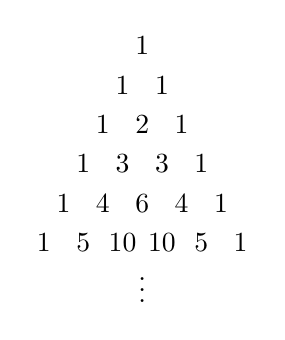
\begin{tikzpicture}[xscale=0.25,yscale=.5]
      \node (00) at ( 0, 0) {$1$};
      \node (10) at (-1,-1) {$1$};
      \node (11) at ( 1,-1) {$1$};
      \node (20) at (-2,-2) {$1$};
      \node (21) at ( 0,-2) {$2$};
      \node (22) at ( 2,-2) {$1$};
      \node (30) at (-3,-3) {$1$};
      \node (31) at (-1,-3) {$3$};
      \node (32) at ( 1,-3) {$3$};
      \node (33) at ( 3,-3) {$1$};
      \node (40) at (-4,-4) {$1$};
      \node (41) at (-2,-4) {$4$};
      \node (42) at ( 0,-4) {$6$};
      \node (43) at ( 2,-4) {$4$};
      \node (44) at ( 4,-4) {$1$};
      \node (50) at (-5,-5) {$1$};
      \node (51) at (-3,-5) {$5$};
      \node (52) at (-1,-5) {$10$};
      \node (53) at ( 1,-5) {$10$};
      \node (54) at ( 3,-5) {$5$};
      \node (55) at ( 5,-5) {$1$};
      \node (d1) at ( 0,-6) {$\vdots$};
    \end{tikzpicture}\\
    \noindent where each number is the sum of the two above, \eg $\binom42 = 6$.}
  \[
    \binom nk \defeq \frac{n!}{k!(n-k)!}.
  \]
  Find a formula for the number of $k$-cycle permutations of $A$
  using factorials and/or binomial coefficients.
\end{xca}

\section{The \texorpdfstring{$m$\th}{mᵗʰ} root:
  \coverings over the components of $\Cyc$}

Let's first give names to some important components of $\Cyc$ that
we have met in previous sections, \eg in \cref{lem:componentsofcoversofS1}.

\begin{definition}\label{def:Cyc-components}
Define $\Cyc_0 \defeq \Cyc_{(\zet,\zs)}$.
\glossary(Cyc0){$\protect\Cyc_0$}{the type of infinite cycles,
\cref{def:Cyc-components}} \index{cycle!infinite}
For each positive $m:\NN$, define $\Cyc_m \defeq \Cyc_{(\bn m,\zs)}$.
\glossary(Cycm){$\protect\Cyc_m$}{the type of cycles of order $m>0$,
\cref{def:Cyc-components}} \index{cycle!of order $m>0$}
We call $\Cyc_0$ and $\Cyc_m$ the \emph{type of infinite cycles}
and \emph{type of $m$-cycles}, respectively.\marginnote{%
The forgetful map from $\Cyc_0$ to $\InfCyc$ is an equivalence. 
Therefore we consider $\Cyc_0$ and $\InfCyc$ as definitionally equal.}
\end{definition}

Recall the equivalence $c : \Sc \we \Cyc_0$ of \cref{def:S1toC}
between the circle and the type of infinite cycles.
In this section, we reinterpret the degree $m$ function $\dg{m}$ as a
map of infinite cycles. In fact $\dg{m}$ makes sense as a map on all cycles,
and we'll use it to begin the classification
of the connected \coverings over $\Cyc_n$, for positive integers $n$.
That's why it's instructive to rephrase connected \coverings over $\Sc$
in terms of cycles, even though they could just be transported 
along the identification $\etop c:\Sc\eqto\Cyc_0$ corresponding to $c$.

Before we do the degree $m$ maps, let's note that the
universal \covering over $\Cyc_0$ is represented by the constant function
$\cst{\pt_0}:\bn 1\to\Cyc_0$, sending the unique element
of $\bn 1$ to $\pt_0\defeq(\zet,\zs):\Cyc_0$, the standard infinite cycle.\footnote{%
  In light of \cref{lem:IdCisZet} we see that the fiber
  of this universal \covering over $(X,t):\Cyc_0$ is (equivalent to) $X$ itself
  -- that's certainly a universal set associated to the
  infinite cycle $(X,t)$!}

For the rest of this section, we fix some positive $m:\NN$.
We now give a description of
the $m$-fold \covering over the circle in terms of cycles.

We proceed as follows.
First we present the answer, a \covering we call $\cdg{m}:\Cyc_0\to\Cyc_0$,
and then we prove that $\dg{m}:\Sc\to\Sc$ and $\cdg{m}:\Cyc_0\to\Cyc_0$
correspond to each other (and to $\pow{m}:\Tot(R_m)\to\Sc$)
under the equivalence $c:\Sc\we\Cyc_0$.

What should we require of $\cdg{m}(X,t)$ for $(X,t):\Cyc_0$?
Well, $\dg{m}:\Sc\to\Sc$ sends $\base$ to $\base$ and $\Sloop$ to $\Sloop^m$;
only the $\Sloop^k$ where $k$ is a multiple of $k$ is in the image of $\dg{m}$.
So we have to find an infinite cycle $(Y,u)$ with ``$u^m$ corresponding to $t$''.
We achieve this by ``stretching'' $X$:
Let $Y$ be $m$ copies of $X$ and let $u$ jump idly from one copy to another except every $m$\th time when $u$ also is allowed to use $t$.
This is illustrated in \cref{fig:root} with the shift by $t$ being
vertical and the movement from copy to copy going around a circle.
\begin{marginfigure}
  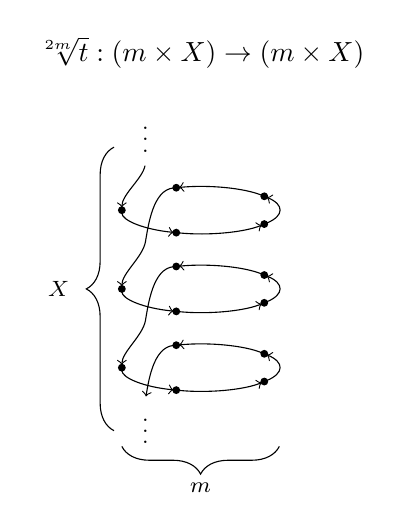
\begin{tikzpicture}
    \node (A) at (0,4) {$\sqrt[\uproot{2}m]t:(\bn m\times X)\to(\bn m\times X)$};
    \foreach \y in {0,1,2}
    { \begin{scope}[shift={(0,\y)}]
        \foreach \x in {0,...,4}
        { \node[fill,circle,inner sep=1pt] at (180+72*\x:1 and .3) {}; }
        \foreach \x in {0,...,3}
        { \draw[->,shorten <=1pt,shorten >=1pt]
          (180+72*\x:1 and .3) arc(180+72*\x:252+72*\x:1 and .3); }
      \end{scope} }
    \foreach \y in {1,2}
    { \begin{scope}[shift={(0,\y)}]
        \draw[->,shorten <=1pt,shorten >=1pt] (108:1 and .3)
        .. controls ++( 5:-.3) and ++(80:.2) .. (-.7,-.4)
        .. controls ++(80:-.2) and ++(90:.2) .. (-1,-1);
      \end{scope} }
    \draw[->,shorten <=1pt,shorten >=1pt] (108:1 and .3)
    .. controls ++( 5:-.3) and ++(80:.2) .. (-.7,-.4);
    \node (dz) at (-.7,-.7) {\footnotesize$\vdots$};
    \begin{scope}[shift={(0,3)}]
      \draw[->,shorten <=1pt,shorten >=1pt] (-.7,-.4)
      .. controls ++(80:-.2) and ++(90:.2) .. (-1,-1);
      \node (da) at (-.7,0) {\footnotesize$\vdots$};
    \end{scope}
    \draw [decorate,decoration={brace,amplitude=10pt}]
    (-1.1,-.8) -- (-1.1,2.8) node [black,midway,xshift=-20pt] {\footnotesize $X$};
    \draw [decorate,decoration={brace,amplitude=10pt}]
    (1,-1) -- (-1,-1) node [black,midway,yshift=-15pt] {\footnotesize $\bn{m}$};
  \end{tikzpicture}
  \caption{The $m$\th root $\sqrt[\uproot{2}m]t$
    of a function $t: X\to X$,
    here illustrated in the case $m=5$.}\label{fig:root}
\end{marginfigure}

\begin{construction}\label{con:root}
  For any type $X$ and $t:X\to X$, we define the $m$\th \emph{root}%
  \glossary(1root){$\protect\mthroot mt$}{$m$\th root function on cycles}
 \[
    {\textstyle\sqrt[\uproot{2}m]t} : (\bn m\times X) \to (\bn m\times X).
  \]
\end{construction}
\begin{implementation}{con:root}
  We set
  \[
    {\textstyle\sqrt[\uproot{2}m]t}(k,x)\defeq
    \begin{cases}
      (k+1,x)& \text{for $k<m-1$ and}\\
      (0,t(x))& \text{for $k=m-1$}.
    \end{cases}
  \]
\par \vspace{-1.5\baselineskip}
\qedhere
\end{implementation}
Only one $m$\th of the time does $\sqrt[\uproot{2}m]t$ use $t:X\to X$,
the rest of the time it applies the successor in $\bn m$.
Indeed, iterating $\sqrt[\uproot{2}m]t$
we get an identification of type $(\sqrt[\uproot{2}m]t)^m(k,x)\eqto(k,t(x))$;
hence the term ``$m$\th root'' is apt.

\begin{definition}\label{def:root}
  The \emph{formal $m$\th root function} is defined by:
  \glossary(917rhom){$\rho_m$}{formal $m$\th root function, \cref{def:root}}
  \[
    \cdg{m}:\sum_{X:\UU}(X\to X)\to\sum_{X:\UU}(X\to X),\qquad
    \cdg{m}(X,t)\defeq(\bn m\times X,{\textstyle\sqrt[\uproot{2}m]t}).\qedhere
  \]
\end{definition}
\noindent We use $\rho$ for ``root'' to denote this incarnation
of the degree $m$ function.

\begin{lemma}\label{lem:root-pres-equiv}
  If $t:X\to X$ is an equivalence,
  then so is $\sqrt[\uproot{2}m]t : (\bn m\times X) \to (\bn m\times X)$.
\end{lemma}
\begin{proof}
  Let $t:X\to X$ be an equivalence. We prove that the fibers of 
  $\sqrt[\uproot{2}m]t$ are contractible.
  
  For the fiber at $(0,x)$ we note,
  using \cref{lem:isEq-pair=}, that identifications in 
  $(0,x)\eqto(\sqrt[\uproot{2}m]t)(\ell,y)$ consist of pairs of proofs 
  of  $\ell=m-1$ and identifications in $x\eqto t(y)$. 
  Both $\sum_{\ell:\bn m}\ell=m-1$ and $t^{-1}(x)$ are contractible,
  and so $(\sqrt[\uproot{2}m]t)^{-1}(0,x)$ is contractible.

  For the fiber at $(k,x)$ with $k:\bn m$ not $0$,
  identifications in $(k,x)\eqto(\sqrt[\uproot{2}m]t)(\ell,y)$
  consist of pairs of proofs of $\ell+1=k$ and identifications in $x\eqto y$,
  so $(\sqrt[\uproot{2}m]t)^{-1}(k,x)$ is contractible since both
  $\sum_{\ell:\bn m}\ell+1=k$ and $\sum_{y:X}x\eqto y$ are.\marginnote{%
    Of course, it's also quite easy to write down an inverse
    of $\sqrt[\uproot{2}m]{t}$ given an inverse of $t$.}
\end{proof}

\begin{lemma} Let $X:\UU$ and $t:X\to X$.
  If $(X,t)$ is a cycle, then so is $\cdg{m}(X,t)$.
\end{lemma}
\begin{proof}
  Clearly, $\bn m\times X$ is a \nonempty set if $X$ is.
  We already know $\sqrt[\uproot{2}m]{t}$ is an equivalence if $t$ is.
  For connectedness, let $(k,x),(k',x'): (\bn m\times X)$.
  We need to show the proposition that there exists $n:\zet$
  with $(k',x') = \bigl(\sqrt[\uproot{2}m]t\bigr)^n(k,x)$.
  Let $n:\zet$ be such that $x' = t^n(x)$.
  Then $(\sqrt[\uproot{2}m]t)^{nm}(k,x) = (k,t^n(x)) = (k,x')$,
  so if $k=k'$ we're done.
  Assume $k<k'$. Then $(\sqrt[\uproot{2}m]t)^{k'-k}(k,x') = (k',x')$,
  so $(\sqrt[\uproot{2}m]t)^{nm+k'-k}(k,x) = (k',x')$, as desired.
  The case $k>k'$ is similar.
\end{proof}

The question now arises: how does $\cdg{m}$ act on the components of $\Cyc$,
and what can we say about the preimages $\cdg{m}^{-1}(X,t)$
for an arbitrary cycle $(X,t)$?

The first part is easy, since the product of $\bn m$ with an $n$-element set
is an $mn$-element set.
\begin{lemma} \label{lem:deg-m-on-Cyc}
  The degree $m$ function restricts to give pointed maps
  \[
    \cdg{m} : \Cyc_n \ptdto \Cyc_{mn} \quad\text{and}\quad
    \cdg{m} : \Cyc_0 \ptdto \Cyc_0.
  \]
\end{lemma}
\begin{proof}
  Recall \cref{def:Cyc-components}. The components $\Cyc_k$ are pointed
  by $\pt_0\defeq(\zet,\zs)$ if $k=0$, and $\pt_k\defeq(\bn k,\zs)$ else.  
  Note\marginnote{%
    In terms of iterated addition, we have
    $\varphi(k,r) = (z \mapsto z+m)^r(k)$.}
  that the function $\varphi : (\bn m\times \zet) \to \zet$
  given by $\varphi(k,r) \defeq k+mr$ is an equivalence,
  with inverse given by Euclidean division by $m$.
  Moreover, we have ${\varphi\!\sqrt[\uproot{2}m]\zs} = {\zs\varphi}$, since
  \[
    \varphi\bigl(\!\sqrt[\uproot{2}m]\zs(k,r)\bigr)
    = k+1+mr = \zs(\varphi(k,r))
    \quad\text{for all $(k,r):\bn m\times \zet$}.
  \]
  This shows that $\varphi$ gives an identification of infinite cycles
  $(\bn m\times\zet, \sqrt[\uproot{2}m]\zs) \eqto (\zet,\zs)$,
  and hence the $m$\th root construction maps the component $\Cyc_0$ to itself.

  Analogously, we can restrict $\varphi$ to
  an equivalence $\bn m \times \bn n \we \sum_{k:\NN}(k<mn)$,
  and get an identification of cycles $\cdg{m}(\pt_n) \eqto \pt_{mn}$,
  showing that $\cdg{m}$ maps the component $\Cyc_n$ to the component $\Cyc_{mn}$.
\end{proof}

We now analyze how $\cdg{m}$ acts on paths.
Let $({\etop{e}},{!}):(X,t)\eqto(X',t')$.
Since $\cdg{m}$ maps first components $X$ to $\bn m\times X$, we get that
the first projection of $\ap{\cdg{m}}({\etop{e}},{!})$ is
${\id\times e} : (\bn m\times X)\eqto(\bn m\times X')$.
We are particularly interested in the case of the loops,
that is, $({\etop{e}},{!}):(X,t)\eqto(X,t)$.
We calculate $(\id\times e)(k,x) = (k,e(x))$,
which by the property of the $m$\th root is equal to $(\sqrt[\uproot{2}m]e)^m(k,x)$.
In particular, if we take $e\defeq t^{-1}$,
then we get $(\id\times t^{-1}) = (\sqrt[\uproot{2}m]{t^{-1}})^m$, which means that
$\ap{\cdg{m}}({\etop{t}^{-1}},{!})$ is indeed the $m$\th power of a
generating loop at the image cycle $\cdg{m}(X,t)$.
In particular, this holds for the standard infinite cycle $(\zet,\zs):\Cyc_0$
and the standard $n$-cycle $(\bn n,\zs):\Cyc_n$.

Why does $\cdg{m}:\Cyc_0\to\Cyc_0$
correspond to the $m$-fold \covering we defined in \cref{def:mfoldS1cover}?
Recall the equivalence $c:\Sc\to C$ from \cref{def:S1toC}.
For the two $m$-fold covers to correspond under this equivalence
we need an element in the identity type represented by
\[
  \begin{tikzcd}
    \Sc\ar[r,"c"]\ar[d,"\dg{m}"'] & \Cyc_0\ar[d,"\cdg{m}"] \\
    \Sc\ar[r,"c"] & \Cyc_0.
  \end{tikzcd}
\]
That is, we need an element in $\cdg{m}c\eqto_{\Sc\to\Cyc_0}c\,\dg{m}$.
Under the equivalence
\[
  \ev_{\Cyc_0}:(\Sc\to\Cyc_0)\we \sum_{(X,t):\Cyc_0}\bigl((X,t)=(X,t)\bigr)
\]
of \cref{lem:freeloopspace},
the composite $c\,\dg{m}$ is given by $\bigl((\zet,\zs),\zs^{-m}\bigr)$
and the composite $\cdg{m}c$ is given by
$\bigl((\bn m\times\zet,\sqrt[\uproot{2}m]{\zs}),\id\times\zs^{-1}\bigr)$:
we must produce an element in
\[
  \Bigl((\bn m\times\zet,\sqrt[\uproot{2}m]{\zs}),\id\times\zs^{-1}\Bigr)
  \eqto \bigl((\zet,\zs),\zs^{-m}\bigr).
\]
Consider the equivalence  $\varphi: (\bn m\times \zet)\we\zet$ with $\varphi(k,n)\defeq k+mn$
also used in \cref{lem:deg-m-on-Cyc}. discussed above.
Transport of $\sqrt[\uproot{2}m]\zs$ along $\varphi$ is exactly $\zs$,
\ie $\varphi\!\sqrt[\uproot{2}m]\zs=\zs\varphi$.\footnote{%
Note that we formulate this in such a way that we don't need to talk about the inverse of $\varphi$.
Of course, the inverse of $\varphi$ maps $z:\zet$ to the remainder and the integer quotient of $z$
under Euclidean division by $m$, cf.~\cref{lem:euclid-div}.}
Likewise, transport of $\id\times\zs^{-1}$ along $\varphi$ is $\zs^{-m}$,
so that $\varphi$ lifts to an element in
$\bigl((\bn m\times\zet,\sqrt[\uproot{2}m]{\zs}), \id\times\zs^{-1}\bigr)
\eqto \bigl((\zet,\zs),\zs^{-m}\bigr)$.

\begin{xca}\label{xca:pointed-maps-circle}
Extend the above construction to an identification of type $\cdg{m}c\eqto_{\Sc\ptdto\Cyc_0}c\,\dg{m}$ 
in case all these maps are taken to be pointed.
\end{xca}

So we know that the fiber of $\cdg{m}$ at an infinite cycle $(X,t)$
is an $m$-element set. In fact, we can identify this set as
$X/m \defeq X/\sim_m$ where $\sim_m$ is the equivalence relation that
identifies points that are a distance $mr$ apart, for some $r:\zet$.
Formally, let $x\sim_m x'$ if and only if $\exists_{r:\zet}(x'=t^{mr}(x))$.
(Such an $r$ is unique if it exists.)
Indeed, the fiber is
\[
  \sum_{(Y,u):\Cyc_0}\bigl((X,t) \eqto (\bn m\times Y, \sqrt[\uproot{2}m]{u})\bigr).
\]
The equivalence is obtained by sending an equivalence class $Y$ of $X/m$ to
the corresponding infinite cycle $(Y,u^m)$ together with the
natural identification $(X,t) \eqto (\bn m\times Y, \sqrt[\uproot{2}m]{u^m})$.
See \cref{thm:fiber-cdg} below for a careful proof of a more general statement.

The reader will no doubt have noticed that $X/m$ is a \emph{finite cycle}.
We'll return to the significance of this below in~\cref{sec:higher-images}.

Our next step is to identify the fiber of $\cdg{m}$ over a general cycle $(X,t)$.
Classically, the remaining cases are those of finite $n$-cycles,
but it's illuminating to be a bit more general.
Note that the equivalence relation $\sim_m$ defined above for an infinite cycle
makes sense for all cycles.

\begin{lemma}\label{lem:sum-cycle-point-contr}
  For any order $d:\Order$, the type $\sum_{(X,t):\Cyc_d}X$ is contractible,
  where $\Cyc_d$ denotes the component of $\Cyc$ consisting
  of cycles of order $d$.
\end{lemma}
\begin{proof}
  This is relatively straight-forward from \cref{lem:IdCycle}.
  The type in question is nonempty since all cycles have a nonempty underlying set,
  so it suffices to prove the type is a proposition.
  So let $(X,t),(X',t')$ be cycles of order $o$, and take $x:X$ and $x':X$.
  An identification of $((X,t),x)$ and $((X',t'),x')$ is given by an identification 
  of cycles $e : (X,t) \eqto (X',t')$ such that $e(x)=x'$.
  But evaluation at $x$ induces an equivalence of type
  $\bigl((X,t) \eqto (X',t')\bigr) \equivto X'$,
  so there exists a unique $e$ with $e(x)=x'$.
\end{proof}
\begin{lemma}\label{lem:m-root-id}
  For any cycle $(X,t)$, if $(\sqrt[\uproot{2}m]{t})^n = \id$,
  then $m$ divides $n$, \ie $n=mq$ for some $q:\zet$, and $t^q=\id$.
  In other words, $m$ divides the order of $\sqrt[\uproot{2}m]{t}$.
\end{lemma}
This follows simply by looking at the first component,
where $\sqrt[\uproot{2}m]{t}$ acts as the successor operation on $\bn m$.

We're almost ready to identify the fiber of $\cdg{m}$ at a cycle $(X,t)$.
We know from \cref{lem:m-root-id} that the fiber
is \nonempty only if $m$ divides the order of $t$.
A key ingredient for the converse is the following.
\begin{lemma}\label{lem:X-mod-m-chosen}
  Let $(X,t):\Cyc$ be a cycle with a chosen point $x_0:X$
  and with order divisible by $m$.
  Then the map $f : \bn m \to X/m$, $f(k) \defeq [t^k(x_0)]$
  is an equivalence.
\end{lemma}
\begin{proof}
  Fix an equivalence class $V:X/m$ and consider its preimage under $f$,
  $f^{-1}(V) \jdeq \sum_{k:\bn m}(V=[t^k(x_0)])$.
  The contractibility of this type is a proposition, so we may choose
  $x:X$ with $V=[x]$.
  Then $(V=[t^k(x_0)])\equiv([x]=[t^k(x_0)])\equiv(x\sim_m t^k(x_0))$.
  So we need to show that $\sum_{k:\bn m}(x\sim_m t^k(x_0))$ is contractible.
  More simply, we need to show that there is a unique $k$ with $x\sim_m t^k(x_0)$.
  Since $(X,t)$ is a cycle, we may further choose $n:\zet$ with $x=t^n(x_0)$.
  By Euclidean division, write $n=qm+r$ with $q:\zet$, $r:\bn m$.
  Then $x = t^n(x_0) \sim_m t^r(x_0)$, so we have our center.
  Let $k:\bn m$ also satisfy $x\sim_m t^k(x_0)$.
  We need to show the proposition $k=r$.
  But $t^{r-k}(x_0) \sim_m x_0$, so we may take $q:\zet$ with $t^{qm+r-k}(x_0)=x_0$.
  Since $m$ divides the order of $t$, this implies $r=k$, as desired.
\end{proof}
Now we have all the pieces needed to prove the main result.
\begin{theorem}\label{thm:fiber-cdg}
  For \emph{any} cycle $(X,t)$, the preimage $\cdg{m}^{-1}(X,t)$
  is equivalent to $P\times X/m$,
  where $P\defeq (m \mid \ord(t)) \jdeq (H_t \subseteq m\zet)$
  expresses that $m$ divides the order of $t$.
\end{theorem}
\begin{proof}
  We'll use \cref{lem:weq-iso}, and we first define the function
  \[
    g : \cdg{m}^{-1}(X,t) \to P\times X/m,
  \]
  by mapping $(Y,u)$ and an identification of cycles
  $e : (X,t) = (\bn m\times Y,\sqrt[\uproot{2}m]{u})$
  to the proof of $P$ from \cref{lem:m-root-id}
  and the class $V_e\defeq [e^{-1}(0,y)]:X/m$, for any $y:Y$.
  Note that this doesn't depend on $y$, so that \cref{thm:wconstant-elim} applies.
  As a subset of $X$, $V_e=\setof{x:X}{\fst(e(x))=0}$.

  In the other direction, to define the function
  \[
    h : P\times X/m \to \cdg{m}^{-1}(X,t),
  \]
  fix an equivalence class $V:X/m$,
  and assume that $m$ divides the order of $t$.
  Then we have, with a bit of abuse of notation, the cycle $(V,t^m)$,
  where we also write $V$ for the type of elements in $X$ that lie in the class $V$,
  and $t^m$ is the restriction of this power of $t$ to $V$.\footnote{%
    If $x$ lies in $V$, then so does $t^m(x)$.}
  We also need an identification
  $(X,t)=(\bn m\times V,\sqrt[\uproot{2}m]{t^m})$.
  This we define via a map $e : \bn m\times V \to X$, $e(k,x) \defeq t^k(x)$.
  This is an equivalence as long as the orders match.
  So let $n:\zet$, and assume first that $t^n=\id$.
  Then $P$ implies that we may write $n=qm$ for some $q:\zet$,
  so
  \[
    (\sqrt[\uproot{2}m]{t^m})^n
    = (\sqrt[\uproot{2}m]{t^m})^{qm}
    = (\id \times t^m)^q = (\id \times t^{qm}) = \id.
  \]
  Conversely, we know from \cref{lem:m-root-id} again,
  that if $(\sqrt[\uproot{2}m]{t^m})^n=\id$,
  then we may write $n=qm$ for some $q:\zet$,
  and $(t^m)^q=\id$, which by \cref{lem:cycle-order-point-ap}
  implies that $t^n = \id$.

  Straight from these definitions, we see that $g\circ h=\id$.
  We leave to the reader to check that $h\circ g=\id$.
\end{proof}

\section{Higher images}
\label{sec:higher-images}

In this section we take a quick break from characterizing the connected \coverings
of $\Cyc_n$ for finite orders $n$ in order to make good on our earlier promise
to say something about the fact that the fiber of $\cdg{m}$, $X/m$, at a cycle $(X,t)$
of order divisible by $m$, itself carries a cycle structure.
This involves the notion of $0$-image of a map, but we might as well introduce the general
notion of $n$-image while we're at it.

Recall from \cref{def:prop-image} the propositional image of a map $f : A \to B$,
  \[
    \im(f) \jdeq \sum_{y:B}\exists_{x:A}(y \eqto f\,x)
           \jdeq \sum_{y:B}\Trunc[\Big]{\sum_{x:A}(y \eqto f\,x)}
           \jdeq \sum_{y:B}\Trunc[\big]{\inv f (y)}.
  \]
We now generalize the propositional image
to higher images, replacing the propositional
truncation involved in the definition by $n$-truncation.

Recall furthermore the image factorization from \cref{xca:unique-fact-image}:
  \[
    \begin{tikzcd}
      A \ar[rr,"f"]\ar[dr,"p"'] & & B \\
      & \im(f)\ar[ur,"i"'] &
    \end{tikzcd}
  \]
Here $p$ is surjective and $i$ is injective, and any such factorization is equivalent to this one. Both surjectivity
(\cref{def:surjection}) and injectivity (\cref{def:injection})
rely on the notion of proposition: all fibers of $p$ are nonempty
and all fibers of $i$ are propositions.

The uniqueness of the factorization $f=ip$ can be visualized
in terms of the two diagonals of the diamond below:
for any surjection $g$ and injection $h$ such that $f=hg$,
that is, the diagram below on the left commutes,
one can construct a (unique) equivalence $e$ such that
the diagram on the right commutes.

\begin{equation}\label{eqn:image-univ-prop}
    \begin{tikzcd}
      & X \ar[dr,"h"] & & & X \ar[dr,"h"] &\\
      A \ar[rr,"f"]\ar[dr,"p"'] \ar[ur,"g"]& & B
&
      A \ar[dr,"p"'] \ar[ur,"g"]& & B  \\
      & \im(f)\ar[ur,"i"'] & & & \im(f)\ar[ur,"i"']\ar[uu, dotted, "e"] &
    \end{tikzcd}
\end{equation}

The existence of a unique equivalence $e$ as above is called the
\emph{universal property of the propositional image}.
Uniqueness of $e$ above also follows from the following two exercises.

\begin{xca}\label{xca:cancel-injection}
Let $A,B,X$ be types and $i:A\to B$ an injection.
Let $i\blank : (X\to A) \to (X\to B)$ be postcomposition with $i$.
Show that $\ap{i\blank}: (f = g) \to (if = ig)$ is an equivalence,
for any $f,g: X\to A$.
\end{xca}
\begin{xca}\label{xca:cancel-surjection}
Let $A,B,Y$ be types and $p:A\to B$ be a surjection.
Let $\blank p : (B\to Y) \to (A\to Y)$ be precomposition with $p$.
Show that $\ap{\blank p}: (f = g) \to (fp = gp)$ is an equivalence,
for any $f,g: B\to Y$.
\end{xca}

We will now define higher images and generalize the notions
of injection and surjection such that a similar
universal property of higher images can be proved.

\begin{definition}\label{def:n-image}
  Let $A,B$ be types and let $f : A \to B$. We define the $n$-\emph{image} of $f$ as
  \glossary(iman){$\protect\im_n(f)$}{the $\protect n$-image of $\protect f$}
  \[
    \im_n(f) \defeq \sum_{b:B}\Trunc{\inv f (b)}_n.\qedhere
  \]
\end{definition}

Observe that $\im_{-1}(f) \jdeq \im(f)$.

\begin{definition}\label{def:n-connected}
  A type $A$ is called $n$-\emph{connected}\index{type!$n$-connected}
  if its truncation $\Trunc A _ n$ is contractible.

  A function $f : A \to B$ is called $n$-\emph{connected}\index{function!$n$-connected}
  if the fiber $\inv f (b)$ is $n$-connected, for each $b:B$.
\end{definition}

Thus, any type is $(-2)$-connected, since its $(-2)$-truncation is contractible.
Moreover, the $(-1)$-connected types are precisely the nonempty ones,
and the $0$-connected types are those we have called connected in \cref{def:connected}.

\begin{definition}\label{def:n-truncated}
  A function $f : A \to B$ is called $n$-\emph{truncated}\index{function!$n$-truncated}
  if the fiber $\inv f (b)$ is an $n$-type, for each $b:B$.
\end{definition}

One may verify now that the $(-1)$-connected functions are the surjections, and
the $(-1)$-truncated functions are the injections.

There is a \emph{factorization} $f = i p$ of a map $f : A \to B$ through its $n$-image,
where $p$ is defined by setting $p(a)\defeq (f(a),\trunc{(a,\refl{f(a)})}_n)$,
and where $i$ is defined by setting $i\defeq\fst$, as in the following diagram.

\begin{equation}\label{eqn:n-image-factorization}
    \begin{tikzcd}
      A \ar[rr,"f"]\ar[dr,"p"'] & & B \\
      & \im_n(f)\ar[ur,"i"'] &
    \end{tikzcd}
\end{equation}

The map $i$ is $n$-truncated, because, for any $b:B$, the fiber $\inv i (b)$ is equivalent to $\Trunc{\inv f (b)}_n$.
Furthermore, by \cref{lem:sum-of-fibers} and the following lemma, $p$ is $n$-connected.

\begin{lemma}\label{lem:trunc-n-connected}
For every type $A$, the constructor $\trunc{\blank}_n : A\to \Trunc{A}_n$
is $n$-connected.
\end{lemma}
\begin{proof}
We have to prove that the $n$-truncation of each fiber of $\trunc{\blank}_n$
is contractible. We start by defining a function
$c:\prod_{x:\Trunc{A}_n} \Trunc{\inv{\trunc{x}}_n}_n$ producing the centers.
Since $c$ takes values in $n$-types, we can define $c$ by
$n$-truncation elimination by setting
$c(\trunc{a}_n) \defeq \trunc{(a,\refl{\trunc{a}_n})}_n$.

The next step is to construct an element of
$\prod_{x:\Trunc{A}_n} \prod_{y:\Trunc{\inv{\trunc{x}}_n}_n} (c(x)=y)$.
Since the identity $c(x)=y$ is an $(n-1)$-type, it suffices to give an element of
$\prod_{x:\Trunc{A}_n} \prod_{z:\inv{\trunc{x}}_n} (c(x)=\trunc{z}_n)$.
Since fibers are sum types,  it suffices to give an element of
$\prod_{x:\Trunc{A}_n} \prod_{a:A} \prod_{p: x=\trunc{a}_n} (c(x)=\trunc{(a,p)}_n)$.
After swapping the first two products, the identity reduces by path induction
to $c(\trunc{a}_n)=\trunc{(a,\refl{\trunc{a}_n})}_n$, for which we can use
the reflexivity path.
\end{proof}

\begin{construction}\label{con:fibcomp=fibfib}
  Let $g:A\to X$ and $h: X\to B$, and let
$\tilde{g}:A\to \sum_{b:B}\inv h (b)$ be the composition of $g$
with the canonical equivalence $X\to \sum_{b:B}\inv h (b)$ from \cref{lem:sum-of-fibers}.
Thus $\tilde{g}(a)\jdeq (h(g(a)),g(a),\refl{h(g(a))})$ for each $a:A$,
and we have the following commutative diagram:
  \[
    \begin{tikzcd}
      A \ar[r,"g"] \ar[dr,"\tilde{g}"'] & X \ar[r,"h"] \ar[d, eqr] & B \\
      & \sum_{b:B}\inv h (b) \ar[ur,"\fst"'] &
    \end{tikzcd}
  \]
Then we have equivalences $e(b) : \inv {(hg)} (b) \equivto \sum_{y:\inv h (b)} \inv {\tilde{g}}(b,y)$
for all $b:B$.
\end{construction}
\begin{implementation}{con:fibcomp=fibfib}
Let, for each $b:B$, $e(b)$ map any pair $(a,p):\inv {(hg)} (b)$ to
$((g(a),p),(a,q))$. Here $q$ is of type $(b,g(a),p) = (h(g(a)),g(a),\refl{h(g(a))})$
and is given componentwise by $p: b=h(g(a))$, $\refl{g(a)}$, and by the
easy path over $p$ from $p$ to $\refl{h(g(a))}$ in the identity type family $\blank=h(g(a))$.
This construction uses \cref{def:pairtopath}, \cref{def:pathover-trp},
and \cref{xca:trp-in-a/x=b/x}\ref{trp-in-x=a}.
\end{implementation}

\begin{xca}\label{xca:fibcomp=fibfib}
Complete the details of \cref{con:fibcomp=fibfib}.
In particular, prove that $e$ is a fiberwise equivalence.
Alternatively, construct your own $e$ by using \cref{cor:contract-away} (twice!).
\end{xca}

\begin{xca}\label{xca:pullout-base-type}
Let $X$ be an $n$-type and let $Y(x)$ be a type for all $x:X$.
Construct canonical equivalences
$\Trunc{\sum_{x:X} Y(x)}_n \to \sum_{x:X} \Trunc{Y(x)}_n$  and
$\Trunc{\prod_{x:X} Y(x)}_n \to \prod_{x:X} \Trunc{Y(x)}_n$.
\end{xca}

We shall now show that the $n$-image factorization
of $f:A\to B$ in \cref{eqn:n-image-factorization} is unique.
This result can be visualized in a similar way as we
did in \cref{eqn:image-univ-prop} for $n=-1$,
and is called the \emph{universal property of the $n$-image}.

\begin{marginfigure}
\noindent\begin{tikzcd}
      & X \ar[dr,"h"] & \\
      A \ar[rr,pos=0.7,"f"]\ar[dr,"p"'] \ar[ur,"g"]& & B\\
      & \im_n(f)\ar[ur,"i"']\ar[uu,dotted,pos=0.3, "e"] &
    \end{tikzcd}
\caption{Universal property of the $n$-image.}
\label{fig:n-image-univ-prop}
\end{marginfigure}

\begin{theorem}\label{thm:n-im-univ-prop}
Let conditions be as in \cref{eqn:n-image-factorization}.
For a given type $X$, assume we are given an $n$-connected
function $g:A\to X$ and an $n$-truncated function $h:X\to B$ with $f=hg$.
Then there exists a unique equivalence $e: \im_n(f)\to X$
such that $g=ep$ and $i=he$.
\end{theorem}

\begin{proof}
We have to construct the equivalence $e$ such that the diagram
in \cref{fig:n-image-univ-prop} commutes; uniqueness of $e$
follows from an easy generalization of \cref{xca:cancel-injection}
and the left triangle in \cref{fig:n-image-univ-prop}.
To simplify this construction,
we are going to replace $g$ and $h$ by projection maps.

In view of \cref{con:fibcomp=fibfib}, we may assume without
loss of generality that $X\jdeq \sum_{b:B} P(b)$ for some
family of $n$-types $P(b)$, and $h\jdeq\fst$.

\begin{marginfigure}
  \noindent\begin{tikzcd}[column sep=tiny]
      &\sum\limits_{b:B} P(b)\ar[rd,"\fst"]\\
      \sum\limits_{b:B} R(b)
        \ar[rd,"{(b,y,q)\mapsto(b,\trunc{(y,q)}_n)}"']
        \ar [ru,"{(b,y,q)\mapsto(b,y)}"]
        \ar [rr,pos=0.7,"\fst"]
      &&B\\
      &\sum\limits_{b:B} \Trunc{R(b)}_n
         \ar [ru,"\fst"']
         \ar [uu,dotted,pos=0.3,"e"']
\end{tikzcd}
\caption{Universal property of the $n$-image, reinterpreted.}
\label{fig:n-im-univ-prop-sumB}
\end{marginfigure}

By \cref{lem:sum-of-fibers} we may also assume without
loss of generality that
$A\jdeq\sum_{b:B}\sum_{y:P(b)} Q(b,y)$, where
$Q(b,y) \defeq\inv g (b,y)$ are the fibers of $g$,
which are all $n$-connected by assumption.
Define $R(b)\defeq\sum_{y:P(b)} Q(b,y)$ for all $b:B$.
With $A\jdeq \sum_{b:B} R(b)$, the function $g$
takes the form of the projection map $(b,y,q)\mapsto(b,y)$,
as shown in \cref{fig:n-im-univ-prop-sumB}.
By $f=hg$ we then get that $f$ is the first projection,
with its $n$-image equivalent to $\sum_{b:B} \Trunc{R(b)}_n$.
The $n$-connected map $p$ then takes the form
$(b,y,q)\mapsto(b,\trunc{(y,q)}_n)$ as shown in
\cref{fig:n-im-univ-prop-sumB}.

Since $B=\sum_{b:B}\bn{1}$, each type in \cref{fig:n-im-univ-prop-sumB}
can be considered to be the sum of a type family parametrized by $b:B$.
For constructing the equivalence $e$ that makes
\cref{fig:n-im-univ-prop-sumB} commute, it suffices to
construct for each $b:B$ the equivalence $e_b$ such that
\cref{fig:n-im-univ-prop-b:B} commutes.
Then we obtain $e$ as desired by summing over $B$, that is,
by putting $e(b,z) \defeq (b,e_b(z))$ for all $b:B$ and $z:\Trunc{R(b)}_n$.

\begin{marginfigure}
  \noindent\begin{tikzcd}
      &P(b)\ar[rd]\\
      R(b)
        \ar[rd,"{\trunc{\blank}_n}"']
        \ar [ru,"{\fst}"]
      &&\bn{1}\\
      &\Trunc{R(b)}_n
         \ar [ru]
         \ar [uu,dotted,"e_b"']
\end{tikzcd}
\caption{Taking summands for $b:B$ in \cref{fig:n-im-univ-prop-sumB}.}
\label{fig:n-im-univ-prop-b:B}
\end{marginfigure}

Now let $b:B$. We have $\Trunc{R(b)}_n \jdeq \Trunc{\sum_{y:P(b)} Q(b,y)}_n$.
By \cref{xca:pullout-base-type}, since $P(b)$ is an $n$-type by assumption,
we have the canonical equivalence
$\Trunc{\sum_{y:P(b)} Q(b,y)}_n\to\sum_{y:P(b)}\Trunc{Q(b,y)}_n$
defined by mapping $\trunc{(y,q)}_n$ to $(y,\trunc{q}_n)$.
For each $y:P(b)$, since $Q(y,b)$ is by assumption $n$-connected,
so that $\Trunc{Q(b,y)}_n = \bn{1}$,
we also have the canonical equivalence $\fst: \sum_{y:P(b)}\Trunc{Q(b,y)}_n \to P(b)$.
The composite of these two equivalences is $e_b$. Regarding the commutation
of \cref{fig:n-im-univ-prop-b:B}, we have $e_b \trunc{\blank}_n \jdeq \fst$
for the left triangle, and the right triangle commutes trivially.

An alternative proof of the uniqueness of $e$ can be obtained
by using the right triangle in \cref{fig:n-im-univ-prop-sumB}.
This reduces the uniqueness of $e$ to the uniqueness of $e_b$
for each $b:B$. The latter follows from the universal property
of $n$-truncation and the left triangle in \cref{fig:n-im-univ-prop-b:B}.
\end{proof}

As an application, we consider the fibers of $m$\th root map
$\cdg{m}$. On infinite cycles, this is equivalent to the degree $m$ map
of the circle by~\cref{xca:pointed-maps-circle}, so we have a map
$\blank/m : \Cyc_0 \to \Set$, which we can identify with the family
$R_m : \Sc \to \Set$ (\cref{def:RmtoS1})
after precomposition with the equivalence
$c : \Sc \to \Cyc_0$ from~\cref{thm:S1bysymmetries}.
For every infinite cycle $(X,t)$, the set $X/m$ has $m$ elements,
so the $(-1)$-image is $\FinSet_m$, the groupoid of $m$-element sets
(\cref{def:groupoidFin}).
But what is the $0$-image?

\begin{theorem}\label{thm:image-Z-to-Cm}
  The $0$-image factorization of the map $\blank/m : \Cyc_0 \to \Set$
  is the composition $p\circ q$, where $q : \Cyc_0 \to \Cyc_m$
  sends the infinite cycle $(X,t)$ to the $m$-cycle $(X/m,\bar t)$,
  where $\bar t : X/m \to X/m$ maps $[x]$ to $[t(x)]$,
  and $p:\Cyc_m\to\Set$ sends an $m$-cycle to its underlying set.
\end{theorem}

\begin{proof}
  We need to check that $q$ is $0$-connected
  and that $p$ is $0$-truncated.

  The latter is direct, since the preimage of $p$ at an $m$-element set $Y$
  is the set of functions $u : Y \to Y$ that make $Y$ into an $m$-cycle.

  To show that $q$ is $0$-connected,
  it suffices to consider the fiber at the standard $m$-cycle $(\bn m,\zs)$.
  We'll show that this fiber is equivalent to $\Cyc_0$ itself, which is indeed $0$-connected.
  The mediating map is induced by our old friend $\cdg{m}$.
  Indeed, define $\varphi : \Cyc_0 \to q^{-1}(\bn m,\zs)$
  by $\varphi(X,t)\defis(\cdg{m}(X,t), r)$,
  where $r$ is the canonical equivalence $(\bn m\times X)/m \equivto \bn m$.
  The inverse of $\varphi$, $\psi$, sends a pair $((Y,u), r)$,
  with $(Y,u):\Cyc_0$ and $r : Y/m \equivto \bn m$
  to $(r^{-1}(0), u^m)$.
\end{proof}

\begin{xca}
  Complete the proof by verifying that $\varphi$ and $\psi$ are indeed mutually inverse.
\end{xca}

The theorem and its proof in fact generalize to all orders.

\begin{xca}\label{xca:image-Cmd-to-Cm}
  Let $d$ be any order and consider the fiber of $\cdg{m}$ on the component
  $\Cyc_{md}$, $\blank/m : \Cyc_{md} \to \Set$.
  Show that the $0$-image factorization of this goes via $\Cyc_m$ by
  lifting $\blank/m$ to $q : \Cyc_{md} \to \Cyc_m$.
  In particular, show that the preimage of $q$ at the standard $m$-cycle
  is equivalent to $\Cyc_d$.
\end{xca}

\section{Universal property of $\Cyc_n$}
\label{sec:universal-property-cyc-n}

This section is devoted to showing that maps out of $\Cyc_n$ into a groupoid $A$
are equivalently given by the choice of a point together with a symmetry of
order $n$: that is any map $\Cyc_n \to A$ is fully determined by a point $a$ together with a symmetry $\sigma:a\eqto a$ such that
$\sigma^n=\refl a$.\footnote{Notice that this is a less general result than the universal property of the circle, or equivalently, the case $n=0$, where we don't need to assume that $A$ is a groupoid.}

Recall that $\Cyc_n$ contains the point $\pt_n \defequi (\bn n, \zs)$,
\ie the standard $n$-cycle. This
point has a symmetry $\sigma_n \defequi (\inv\zs, !)$ whose second projection is a
proof that $\zs\inv\zs = \inv\zs\zs$.
%
Recall also from \cref{cor:id-m-cycle} that all elements of $\pt_n = \pt_n$ are
of the form $\sigma_n^i$ for $i=0,\dots,n-1$.

Given a groupoid $A$, and a map $f :
\Cyc_n \to A$, one can consider $f(\pt_n):A$ and $\ap f (\sigma_n): f(\pt_n) =
f(\pt_n)$. The equation $\refl {\pt_n} = \sigma_n^n$ in
$\Cyc_n$ is mapped by $f$ to a proof of $\refl {f(\pt_n)} =
\ap f(\sigma_n)^n$. Hence, the following map is well defined:
\begin{displaymath}
  \ev_{n,A} : (\Cyc_n \to A) \to \sum_{a:A}\sum_{\sigma:a\eqto a}\refl a = \sigma^n,\quad
  f \mapsto (f(\pt_n), \ap f (\sigma_n), !)
\end{displaymath}

\begin{theorem}
  For any groupoid $A$, the map $\ev_{n,A}$ is an equivalence.
  \label{prop:ump-cycn-into-groupoids}
\end{theorem}
\begin{proof}
  Let $a:A$ and $\sigma:a\eqto a$ be such that $\refl a = \sigma^n$ holds.
  We want to prove that the fiber
  \begin{displaymath}
    \sum_{f:\Cyc_n \to A} (a,\sigma, !) \eqto \ev_{n,A}(f)
  \end{displaymath}
  is contractible. Hence we first need to craft a function $f:\Cyc_n \to A$
  together with $p:a\eqto f(\pt_n)$ such that $\ap f (\sigma_n) \cdot p = p
  \cdot \sigma$.

  In order to do so, we will craft a function $f:\Cyc_n \to A$ together with a
  function $\hat p_x: \pt_n \eqto x \to a \eqto f(x)$ for each $x:\Cyc_n$ such that
  $\hat p_x(\blank\sigma_n) = \hat p_x(\blank) \sigma$. By setting $p \jdeq \hat
  p_{\pt_n}(\refl {\pt_n})$, we would have succeeded. Indeed, path induction on
  $\alpha: x \eqto x'$ shows that $\hat p_{x'}(\alpha \blank) = \ap f (\alpha) \hat
  p_x(\blank)$ on one hand, and the hypothesis on $\hat p$ proves that $\hat
  p_{\pt_n} (\blank) \sigma = \hat p_{\pt_n}(\blank \sigma_n)$ on the other
  hand. This leads to the chain of equations:
  \begin{align*}
    p \sigma &= \hat p_{\pt_n}(\refl {\pt_n}) \sigma
               = \hat p_{\pt_n}(\refl {\pt_n}\sigma_n)
               = \hat p_{\pt_n}(\sigma_n\refl {\pt_n}) \\
             &= \ap f (\sigma_n) \hat p_{\pt_n}(\refl {\pt_n})
               = \ap f (\sigma_n) p
  \end{align*}

  It remains to craft the promised $f$ and $\hat p$. For each $x:\Cyc_n$, consider the type
  \begin{displaymath}
    T(x) \defequi \sum_{b:A}\sum_{\pi: \pt_n \eqto x \to a \eqto b}
    \pi(\blank\sigma_n) = \pi(\blank) \sigma
  \end{displaymath}
  We claim that $T(x)$ is contractible. To prove this proposition for $x$
  ranging over the connected type $\Cyc_n$, it is enough to only prove it for
  $x \jdeq \pt_n$. However, as $i \mapsto \sigma_n^i$ provides an equivalence
  $\bn n \to (\pt_n = \pt_n)$, we get:
  \begin{displaymath}
    T(\pt_n) \weq \sum_{b:A}\sum_{\pi: \bn n \to a \eqto b} \pi(\blank + 1) = \pi(\blank)\sigma
  \end{displaymath}
  Now, note that $\pi:\bn n \to a\eqto b$ such that $\pi(\blank +1) = \pi(\blank)
  \sigma$ is entirely determined by $\pi(0)$, as then $\pi(i) = \pi(0)\sigma^i$
  for all $i:\bn n$. Moreover, an element $q$ in $a\eqto b$ defines a function
  $\pi_q:i \mapsto q\sigma^i$ which satisfies the equation $\pi_q( \blank +1) =
  \pi_q(\blank)q$. In other words, we have an equivalence:
  \begin{displaymath}
    \left( \sum_{\pi:\bn n \to {a\eqto b}} \pi(\blank +1) = \pi(\blank )\sigma \right)
    \equivto
    (a \eqto b), \quad
    (\pi, !) \mapsto \pi(0).
  \end{displaymath}
  Hence, we can simplify further $T(\pt_n)$:
  \begin{displaymath}
    T(\pt_n) \weq \left(\sum_{b:A} a \eqto b\right) \weq 1
  \end{displaymath}
  We then get $f(x)$ by selecting a center of contraction for each $x:\Cyc_n$, and
  the function $\hat p_x$ is then defined as the first projection of the second
  component of this center of contraction.
  %
  \marginnote{The construction of $f$ is really an ad hoc version of the delooping of the abstract group morphism $\sigma_n^i \mapsto \sigma^i$. If we move this section forward, one can rewrite it as such.}


  Finally, we prove that the fiber $\inv{\ev_{n,A}}(a,\sigma,!)$ is a
  proposition. As we just proved that it is inhabited, we would have
  successfully shown that the fiber is contractible. Given two elements
  $(f,p,!)$ and $(f',p',!)$ of the fiber, we want to find a path between the
  two, that is $\chi:\prod_{x:\Cyc_n} f(x) \eqto f'(x)$ such that the following
  commutes:
  \begin{displaymath}
    \begin{tikzcd}
      a \rar[eqr,"p"] \dar[eql,"p'"'] & f(\pt_n) \dlar[eqr,"\chi(\pt_n)"]\\
      f'(\pt_n) &
    \end{tikzcd}
  \end{displaymath}
  Let us denote $U(x)\defequi f(x) \eqto f'(x)$ for $x:\Cyc_n$, and notice that
  these types are sets (as $A$ is a groupoid). The element $\tau\defequi p'\inv
  p : U(\pt_n)$ is peculiar in that  $\trp[U] q (\tau) = \tau$ for all $q:\pt_n\eqto\pt_n$.
  Indeed, we use once
  again that symmetries of $\pt_n$ in $\Cyc_n$ are of the form $\sigma_n^i$ and
  we calculate:
  \begin{displaymath}
    \trp[U] {\sigma_n^i} (\tau) = \ap {f'} (\sigma_n^i) \cdot \tau \cdot \inv{\ap {f}(\sigma_n^i)}
    = p' \sigma^i \inv {p'} \cdot p'\inv p p \sigma^{-i} \inv p = p' \inv p
  \end{displaymath}
  Now it is easy to prove that the following type is contractible:
  \begin{displaymath}
    V(x) \defequi \sum_{\alpha: U(x)} \alpha = \trp[U] \blank (\tau).
  \end{displaymath}
  To do so, we use the connectedness of $\Cyc_n$ and verify the contractibility
  of $V(\pt_n)$ by pointing out that $V(\pt_n)$ is simply the singleton type of
  $\tau$. Now $\chi$ is defined as the function mapping $x$ to the center of
  contraction of $V(x)$. By definition, $\chi(\pt_n) = \tau$ as we wanted.
  %
  \marginnote{The construction of $\chi$ is really an ad hoc version of the following fact: for any $G$-set $X$, the type of fixed points of $X$ is equivalent to the type of sections of $\sum_{z:\BG}X(z) \to \BG$. If we move this section forward, one can rewrite it as such.}
\end{proof}

As a direct corollary, we can classify the connected \coverings over $\Cyc_n$ for finite orders $n$.
Indeed, the corresponding families $S : \Cyc_n \to \Set$ are precisely those cycles $(X,t)$
with $t^n=\id$, \ie whose order divides $n$.
If we restrict to decidable connected \coverings, equivalently, decidable cycles,
these are the usual finite cycles with order dividing $n$.

\section{Getting our cycles in order}
\label{sec:cycles-order}

{\color{casblue} TODO: Exposition and figures

\begin{xca}
  Prove that if $(X,t),(Y,u)$ are cycles, $x_0:X$,
  then the type of maps $f : (X,t) \to (Y,u)$ is equivalent to $P\times Y$,
  where $P\defeq(\ord(u) \mid \ord(t)) \jdeq (H_t \subseteq H_u)$.
\end{xca}

Thus, an order $p$ divides an order $q$ if and only if
there is a map of cycles from a cycle of order $q$
to a cycle of order $p$.
\begin{theorem}
  The partially ordered set $(\Order,|)$ is a lattice
  with least element the finite order $1$
  and greatest element the infinite order, represented by the number $0$,
  and meets and joins given by “gcd” and “lcm”, respectively.
\end{theorem}

subgroups of $\CG_n$: $\CG_k$ where $k | n$,
connected set bundles of $\Cyc_n$.

\subsection{More TODO}

\begin{itemize}
\item Classify connected \coverings over $\Cyc_n$.
\item Universal property of $\Cyc_n$ among groupoids.
\item Bijective proof of $mn = \lcm(m,n)\times\gcd(m,n)$ via the product of cycles.
  Chinese remainder stuff.
\item Somehow sneak in totatives and automorphisms of cyclic groups?
\end{itemize}
}


%%% Local Variables:
%%% mode: latex
%%% TeX-master: "book"
%%% End:
